\documentclass[12pt,aps,pra,reprint,showkeys]{revtex4-1}

\usepackage{amsmath}
\usepackage{amssymb}
\usepackage{array}
\usepackage{booktabs}
\usepackage{charter}
\usepackage[T1]{fontenc}
\usepackage{graphicx}
\usepackage[hidelinks]{hyperref}
\usepackage[utf8]{inputenc}
\usepackage{natbib}
\usepackage{titlesec}
\usepackage{xcolor}

% set bibliography preferences (\requires{natbib})
\bibliographystyle{apalike}
\setcitestyle{authoryear,open={(},close={)}}
\setlength{\bibsep}{1.5\itemsep plus 0.3ex}

% figure controls
\graphicspath{{figures/}}
\renewcommand{\figurename}{Figure}

% increase space between section headings + text (\requires{titlesec})
\titlespacing{\section}{1.5pt}{1\baselineskip}{\baselineskip}
\titlespacing{\subsection}{1.5pt}{1\baselineskip}{\baselineskip}
\titlespacing{\subsubsection}{1.5pt}{1\baselineskip}{\baselineskip}
\urlstyle{same}

% arabic table numbering
\renewcommand{\thetable}{\arabic{table}}

% reset figure / table counts for supplement
\newcommand{\beginsupplement}{
  \setcounter{equation}{0} \renewcommand{\theequation}{S\arabic{equation}}
  \setcounter{table}{0} \renewcommand{\thetable}{S\arabic{table}}
  \setcounter{figure}{0} \renewcommand{\thefigure}{S\arabic{figure}}
}

% no "and" in title affiliations
\renewcommand{\andname}{\ignorespaces}

% modify booktabs lines (\requires{booktabs})
\setlength{\heavyrulewidth}{0.2ex}
\setlength{\lightrulewidth}{0.1ex}

\begin{document}

\title{Comparing spatially-constrained null models for parcellated brain maps}
\author{Ross D. Markello$^{1,*}$}
\author{Bratislav Misic$^{1,*}$}

\affiliation{$^1$McConnell Brain Imaging Centre, Montr\'{e}al Neurological Institute, McGill University, Montr\'{e}al, Canada}
\affiliation{$^{*}$Correspondence to:
    \href{mailto:ross.markello@mail.mcgill.ca}{ross.markello@mail.mcgill.ca} or
    \href{mailto:bratislav.misic@mcgill.ca}{bratislav.misic@mcgill.ca}
}

\begin{abstract}
\noindent Technological and data sharing advances have led to a proliferation of high-resolution structural and functional maps of the brain.
Modern neuroimaging research increasingly depends on identifying correspondences between the topographies of these maps; however, most standard methods for statistical inference fail to account for their spatial properties.
Recently, multiple methods have been developed to generate null distributions that preserve the spatial autocorrelation of brain maps and yield more accurate statistical estimates.
Here, we comprehensively assess the performance of ten such published null frameworks in controlling the family-wise error rate in statistical analyses of parcellated neuroimaging data.
We apply each framework on two prototypical analyses: (1) testing the correspondence between brain maps (e.g., correlating two activation maps) and (2) testing the spatial distribution of a feature within a partition (e.g., quantifying the specificity of an activation map within an intrinsic functional network).
In agreement with previous reports, we find that naive null models that do not preserve spatial autocorrelation consistently yield unrealistically liberal statistical estimates.
Performance of spatially-constrained null models depended on research context; model performance was generally consistent when testing correspondences between brain maps, but considerably more variable when testing partition specificity.
Throughout these analyses, we observe minimal impact of parcellation and parcel resolution on null model performance.
Altogether, our results highlight the need for continued development and standardization of statistically-rigorous methods for comparing brain maps.

\end{abstract}

\keywords{null models | spin test | brain parcellations | spatial autocorrelation | significance testing}

\maketitle

\section*{INTRODUCTION}

The brain is organized as a series of nested and increasingly multi-functional neural circuits.
The connections and interactions among these circuits ultimately manifest as unique topographic distributions of multiple structural and functional properties.
Recent advances in imaging, tracing, and recording technologies \citep{insel2013science}, together with global data sharing initiatives \citep{vanessen2013neuroimage, poldrack2013frontneuroinf, sudlow2015plosmed, casey2018devcogneuro}, have resulted in the generation of high-resolution maps of many of these properties, including gene expression \citep{hawrylycz2012nature, akbarian2015nature}, cytology \citep{voneconomo1925cytoarchitecture, scholtens2018neuroimage}, receptor densities \citep{beliveau2017jneuro, norgaard2020biorxiv, zilles2004janatomy, zilles2009curropneuro}, intracortical myelin \citep{burt2018natneuro, whitakervertes2016pnas}, and functional organization \citep{murray2014natneuro, yeo2011organization, shafiei2020biorxiv, margulies2016pnas, damoiseaux2006pnas, bellec2010neuroimage}.

Increasingly, modern scientific discovery in neuroimaging research depends on identifying correspondences between the topographies of brain maps \citep{baum2020pnas, vazquezrodriguez2019pnas, wang2019sciadvances, shafiei2020biorxiv, gao2020biorxiv, demirtas2019neuron, hansen2020biorxiv}; however, standard methods for statistical inference fall short when making such comparisons \citep{alexander2013convergence, alexanderbloch2018neuroimage, burt2020neuroimage, fulcher2020biorxiv}.
Namely, in spatially-embedded systems---like the brain---neighboring data points are not statistically independent, violating the assumptions of many common inferential frameworks.
As an example, consider computing a correlation between two brain maps.
When using a standard parametric null (i.e., the Student's \textit{t}-distribution), the spatial autocorrelation of the maps violates the inherent requirement that the model errors are independent and identically distributed (\textit{i.i.d.}).
When using a standard non-parametric null (i.e., random permutations of one of the feature maps), the spatial autocorrelation violates the requirement of exchangeability.
In both instances, the calculated $p$-value will be inflated, yielding increased family-wise error rates (FWER, or type 1 error rates) across analyses.

In the past several years multiple frameworks have been developed to overcome the shortcomings of standard null models in neuroimaging.
These frameworks generate null distributions that preserve the spatial autocorrelation of brain maps, yielding statistical inferences that more accurately reflect the underlying data.
Such spatially-constrained null models fall into two broad families: non-parametric spatial permutation models \citep{alexander2013convergence, alexanderbloch2018neuroimage} and parameterized data models \citep{burt2018natneuro, burt2020neuroimage, vosdewael2020brainspace}.
In non-parametric spatial permutation models, the cortical surface is represented as a sphere to which random rotations are applied, generating surface maps with randomized topography but identical spatial autocorrelation.
In parameterized data models, spatial autocorrelation is estimated from the empirical brain maps and used to generate surrogate nulls with randomized topography and similar---though not identical---spatial autocorrelation.
Since their development, these models have been adapted by several researchers \citep{baum2020pnas, cornblath2019arxiv, vasa2018cercor, vazquezrodriguez2019pnas}; to our knowledge, there have been at least ten distinct implementations of null frameworks applied to statistical estimates of brain maps.

The earliest implementations of these null models, proposed in \citet{alexander2013convergence} and later formalized in \citet{alexanderbloch2018neuroimage}, described a non-parametric method by which the cortical surface was subjected to spatial rotations.
The principal challenge of implementing this method is that the medial wall---for which most brain maps contain no data---can be rotated into the cortical surface.
This is an important consideration for parcellated brain maps in particular, because the loss of data caused by this medial wall rotation can bias results.
To address this problem, researchers have opted to either discard the missing data \citep{baum2020pnas, cornblath2019arxiv}, assign the nearest data to missing parcels \citep{vazquezrodriguez2019pnas}, or ignore the medial wall entirely \citep{vasa2018cercor}.
Other groups have devised alternative methods that do not rely on spatial rotations but use generative models instead.
These parameterized frameworks vary in their conceptualization and implementation of the data-generating process, ranging from a spatial lag model \citep{burt2018natneuro} to spectral randomization \citep{wagner2015generating, vosdewael2020brainspace} to variogram matching \citep{burt2020neuroimage}.
How these different models perform when applied to the same experimental questions and datasets remains unclear.

Here, we comprehensively compare how ten published null frameworks control the FWER in statistical analyses of parcellated neuroimaging data.
Using multiple open-access datasets (Neurosynth [\citealt{yarkoni2011natmethods}]; Human Connectome Project [\citealt{vanessen2013neuroimage}]), we apply each framework on two prototypical analyses: (1) assessing the correspondence between brain maps (e.g., correlating two activation maps) and (2) assessing the spatial distribution of a feature within a partition (e.g., quantifying the enrichment of T1w/T2w ratios in resting state networks).
In both analyses we systematically examine the impact of parcellation---which differentially modifies the spatial structure of the underlying data---on the performance of the null frameworks.

\begin{table*}[htp]
    \caption{
      \textbf{Null model frameworks | }
      Overview of the null frameworks and the implementations used in the reported analyses.
      The \emph{Description} column indicates the primary point of methodological divergence for each framework.
      The \emph{Duplications} column indicates whether parcel values can be duplicated in the given framework.
      The \emph{Citation} column indicates the first appearance of the described implementation in the neuroimaging literature, if known.
      Code and/or references to code for implementing all frameworks is available at \url{https://github.com/netneurolab/markello_spatialnulls}.
      \vspace{-0.5\baselineskip}
    }
    \label{table-null-models}
    \setlength{\tabcolsep}{4.5pt}
    \renewcommand{\arraystretch}{1.25}
    \begin{center}
      \begin{tabular}{p{0.15\linewidth} p{0.43\linewidth} p{0.10\linewidth} p{0.25\linewidth}}
                                                                                                                                                                         \toprule
        \multicolumn{4}{c}{\textbf{Naive models}}                                                                                                                     \\ \toprule
        \emph{Method}   & \emph{Description}                                                                                & \emph{Duplications} & \emph{Citation}   \\ \midrule
        Parametric      & Uses standard ``normal'' distributions (e.g., Student's \emph{t}-distribution)                    & No  &                                   \\
        Non-parametric  & Reorders parcels randomly, not taking into account their inherent spatial structure               & No  &                                   \\ \toprule
        \multicolumn{4}{c}{\textbf{Spatial permutation models}}                                                                                                       \\ \toprule
        \emph{Method}   & \emph{Description}                                                                                & \emph{Duplications} & \emph{Citation}   \\ \midrule
        V{\'a}zquez-Rodr{\'i}guez & Assigns parcel centroid to closest rotated centroid based on minimum Euclidean distance & Yes & \citet{vazquezrodriguez2019pnas}  \\
        V{\'a}{\v{s}}a  & Uses an iterative procedure to uniquely assign parcels based on distance to the rotated parcels   & No  & \citet{vasa2018cercor}            \\
        Hungarian       & Uses the Hungarian algorithm to match original and rotated parcel centroids                       & No  &                                   \\
        Baum            & Projects parcel data to vertices, rotates, and takes the mode of vertices in each parcel          & Yes & \citet{baum2020pnas}              \\
        Cornblath       & Projects parcel data to vertices, rotates, and takes the mean of vertices in each parcel          & Yes & \citet{cornblath2019arxiv}        \\ \toprule
        \multicolumn{4}{c}{\textbf{Parameterized data models}}                                                                                                        \\ \toprule
        \emph{Method}   & \emph{Description}                                                                                & \emph{Duplications} & \emph{Citation}   \\ \midrule
        Burt-2018      & Uses a distance-dependent spatially autoregressive model to generate nulls                         & No  & \citet{burt2018natneuro}          \\
        Burt-2020      & Uses a variogram model to estimate spatial autocorrelation to generate nulls                       & No  & \cite{burt2020neuroimage}         \\
        Moran           & Uses a distance-dependent eigendecomposition to generate nulls                                    & No  & \citet{vosdewael2020brainspace}   \\
      \end{tabular}
    \end{center}
\end{table*}

\begin{figure*}[htp]
  \begin{center}
    \centerline{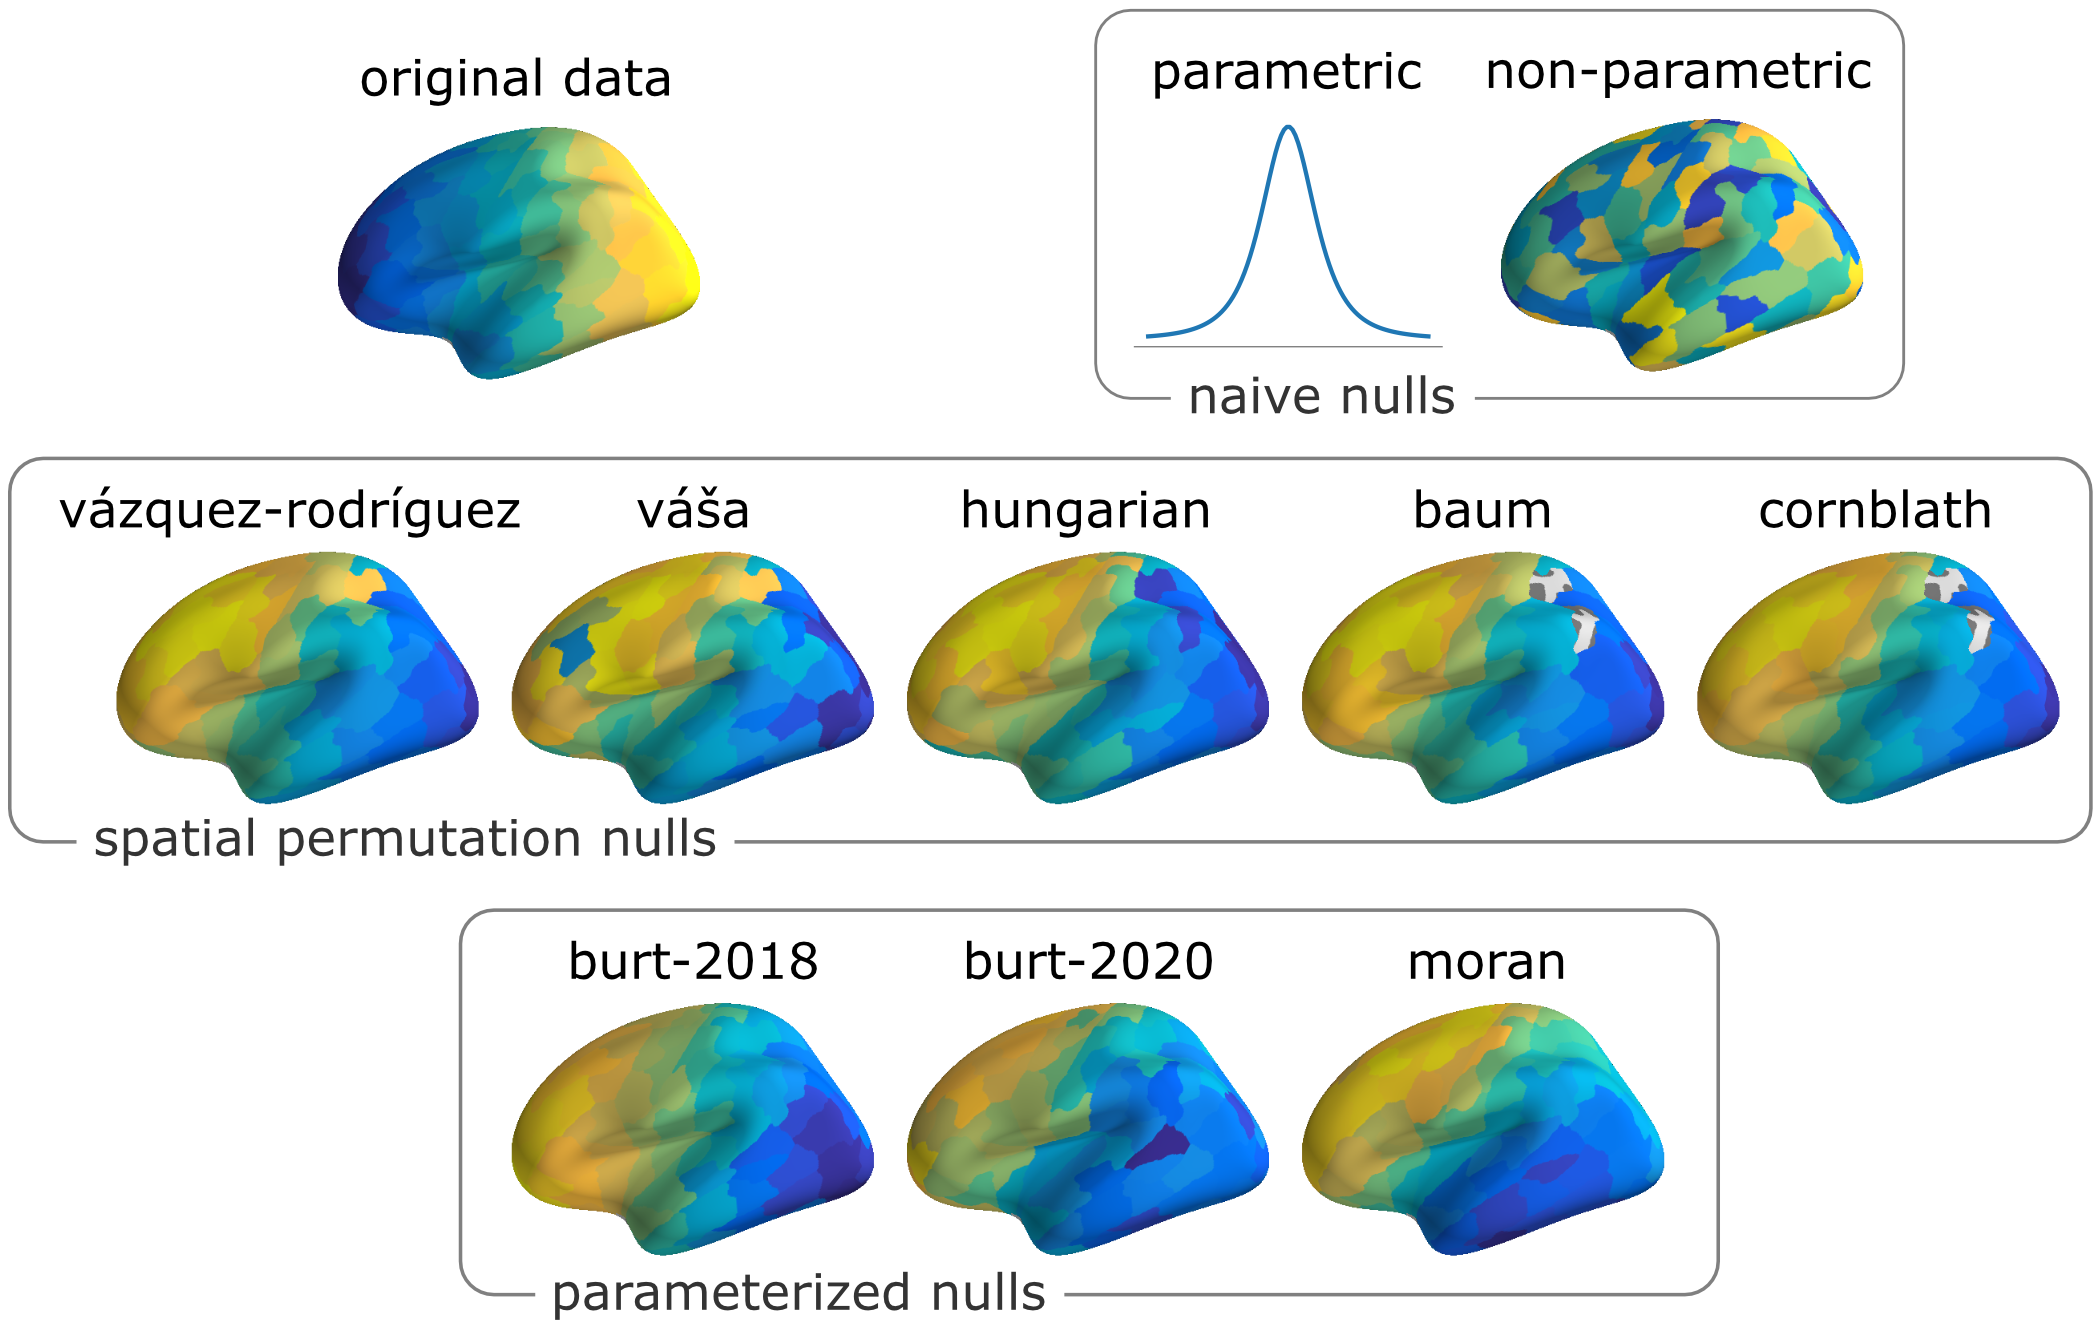
\includegraphics[width=0.9\textwidth]{null-frameworks.png}}
    \caption{
      \textbf{Null model framework examples |}
      Examples of the null frameworks applied to toy data representing an anterior-posterior gradient (original data, top left) using the Cammoun 219-parcel atlas.
      All spatial permutation null examples were generated using the same rotation matrix to highlight variations between the different implementations.
      Parameterized null examples were chosen so as to maximize similarity to the spatial permutation nulls for visualization.
      }
    \label{figure-null-frameworks}
  \end{center}
\end{figure*}

\section*{METHODS AND MATERIALS}

\subsection*{Code and data availability}

All code used for data processing, analysis, and figure generation is available on GitHub (\url{https://github.com/netneurolab/markello_spatialnulls}) and directly relies on the following open-source Python packages: BrainSMASH \citep{burt2020neuroimage}, BrainSpace \citep{vosdewael2020brainspace}, IPython \citep{ipython}, Jupyter \citep{jupyter}, Matplotlib \citep{matplotlib}, NeuroSynth \citep{yarkoni2011natmethods}, NiBabel \citep{nibabel}, NumPy \citep{numpyv1, numpyv2}, Pandas \citep{pandas}, PySurfer \citep{pysurfer}, Scikit-learn \citep{sklearn}, SciPy \citep{scipy}, and Seaborn \citep{seaborn}.
Additional software used in the reported analyses includes FreeSurfer (v6.0.0; \url{http://surfer.nmr.mgh.harvard.edu/}; \citealt{fischl1999humanbrainmap}) and the Connectome Workbench (v1.4.2; \url{https://www.humanconnectome.org/software/connectome-workbench}; \citealt{marcus2011frontiers}).

\subsection*{Data}

\subsubsection*{NeuroSynth association maps}

To replicate the analyses described in \citet{alexanderbloch2018neuroimage} we downloaded ``association'' maps from NeuroSynth \citep{yarkoni2011natmethods} for $t = 123$ terms overlapping with those defined in the Cognitive Atlas (\url{https://www.cognitiveatlas.org/concepts}; \citealt{poldrack2011neuron, poldrack2016annrevpsych}; refer to Table~\ref{supp-table-ns-terms} for a full list of terms).
This resulted in 123 volumetric statistical maps which were then inflated to a mid-gray projection of FreeSurfer's fsaverage5 surface using nearest neighbor interpolation.

\subsubsection*{Human Connectome Project}

Group-averaged T1w/T2w (a proxy for intracortical myelin) data were downloaded from the S1200 release of the Human Connectome Project (HCP; \citealt{vanessen2013neuroimage}).
To ensure consistency with the reported NeuroSynth analyses, data were resampled to FreeSurfer's fsaverage5 surface following instructions on the Human Connectome Project Wikipedia page (\url{https://wiki.humanconnectome.org/display/PublicData/HCP+Users+FAQ}).

\subsubsection*{Brain parcellations}

In order to examine the impact of parcellations on the tested null models we used two multi-scale resolution atlases generated from structural \citep{cammoun2012mapping} and functional \citep{schaefer2018cercor} connectivity data.
The former, referred to throughout the text as the ``Cammoun atlas'', has five resolutions ranging from 68 to 1000 parcels (68, 114, 219, 448, and 1000 parcels), generated by dividing the Desikan-Killiany atlas \citep{desikan2006automated} into equally-sized sub-units based on group-level diffusion weighted imaging data.
The latter, referred to throughout the text as the ``Schaefer atlas'', has ten resolutions ranging from 100 to 1000 parcels in steps of 100 parcels (i.e., 100, 200, 300, and so on), generated via a gradient-weighted Markov Random Field model from resting state fMRI data \citep{schaefer2018cercor}.

NeuroSynth activation maps and the HCP T1w/T2w brain map were parcellated using all resolutions of the Schaefer and Cammoun atlases.
Values for vertices lying on the medial wall of the surface mesh were not considered.

\subsubsection*{Network partitions}

To investigate the partition specificity of brain maps we applied two common network definitions: the seven functional networks defined in \citet{yeo2011organization} and the seven cytoarchitectonic classes proposed by \citet{voneconomo1925cytoarchitecture}.

For the Cammoun atlas we used the fsaverage5 vertex-level Yeo network assignments provided by FreeSurfer.
To derive parcel-wise network assignments from this vertex representation we applied a winner-take-all approach; that is, the mode of the vertices in each parcel was used to select the representative network.
For the Schaefer atlas we used the parcel assignments for the Yeo networks provided by the original authors.
To derive von Economo--Koskinas classes for parcels in both the Cammoun and Schaefer atlases we applied the classifiers provided by \citet{scholtens2018neuroimage} to the fsaverage5 surface, yielding vertex-level assignments; these assignments were then used with the winner-take-all approach to generate parcel-level network assignments.

\subsection*{Null model frameworks}

Here, we briefly describe null model frameworks as initially proposed in the literature, and then explain the specific details of the implementations used in the current report.
For a summary overview of the implementations please refer to Table~\ref{table-null-models}.

\subsubsection*{Naive models}

Commonly used in the neuroimaging literature prior to the development of spatially-constrained frameworks, so-called naive models do not take into account the spatial structure of the data when constructing null distributions, commonly resulting in inflated family-wise error rates.
We test two such models: a \emph{parametric} and a \emph{non-parametric} method.

\paragraph*{Naive parametric method.}

Although the exact implementation of the parametric method varies based on the statistical test employed, all implementations share a reliance on standard null distributions.
For example, when examining correlation values, the parametric method relies on the Student's \emph{t}-distribution; when examining z-statistics, this method uses the standard normal distribution.

\paragraph*{Naive non-parametric method.}

The naive non-parametric approach uses a random permutation (i.e., reshuffling) of the data to construct a null distribution, destroying its inherent spatial structure.
Each parcel is uniquely reassigned the value of another parcel for every permutation.

\subsubsection*{Spatial permutation models}

First published in \citet{alexander2013convergence} and later formalized in \citet{alexanderbloch2018neuroimage}, spatial permutation models generate spatially-constrained null distributions by applying random rotations to spherical projections of the brain.
A rotation matrix ($\mathbf{R}$) is applied to the three-dimensional coordinates of the brain ($\mathbf{V}$) to generate a set of rotated coordinates ($\mathbf{V_{rot}} = \mathbf{V} \mathbf{R}$); the permutation is constructed by replacing the original values at each coordinate with those of the closest rotated coordinate.
Rotations are generated independently for one hemisphere and then mirrored across the anterior-posterior axis for the other.

At the time of writing, we are aware of four published adaptations of this spatial permutation framework that have been applied to parcellated brain data: \citet{vazquezrodriguez2019pnas}, \citet{vasa2018cercor}, \citet{baum2020pnas}, and \citet{cornblath2019arxiv}.
We test all four of these adaptations, in addition to one other method (\emph{Hungarian}) that we posit is a natural extension thereof.

\paragraph*{V{\'a}zquez-Rodr{\'i}guez method.}
The \textit{V{\'a}zquez-Rodr{\'i}guez} method, which serves as a direct adaptation of the original framework from \citet{alexanderbloch2018neuroimage} but applied to parcellated brain data, was first used in \citet{vazquezrodriguez2019pnas}.
In this adaptation, vertex coordinates are replaced with those of parcel centroids.
That is, a rotation is applied to the coordinates for the center-of-mass of each parcel, and parcels are reassigned the value of the closest rotated parcel (i.e., that with the minimum Euclidean distance).
As in the original formulation this method permits the duplicate reassignment of parcel values for every rotation, such that some parcel values may not be present in a given rotation and others may appear more than once.

\paragraph*{V{\'a}{\v{s}}a method.}

The first known application of spatial permutations to parcellated data, the \textit{V{\'a}{\v{s}}a} method \citep{vasa2018cercor} attempted to resolve the primary issue of the Alexander-Bloch method: duplicate reassignments.
That is, this method was created so as to yield a perfect permutation of the original data for every rotation.
As with the \textit{V{\'a}zquez-Rodr{\'i}guez} method, parcel centroids are used instead of vertex coordinates.
In order to avoid duplicate reassignments, parcels are iteratively assigned by (1) finding the closest rotated parcel to each original parcel, and (2) assigning the most distant pair of parcels.
This two-step process is then repeated for all remaining unassigned parcels until each has been reassigned.

\paragraph*{Hungarian method.}

Similar to the \textit{V{\'a}{\v{s}}a} method, the \textit{Hungarian} method attempts to uniquely reassign each parcel for every rotation.
Instead of using an iterative process, however, which can result in globally sub-optimal assignments, this method uses the Hungarian algorithm to solve a linear sum assignment problem \citep{kuhn1955hungarian}.
This method attempts to uniquely reassign each parcel such that the global reassignment cost is minimized, where cost is quantified as the distance between the original and rotated parcel centroid coordinates.

\paragraph*{Baum method.}

Used initially in \citet{baum2020pnas}, this method projects parcellated brain data to a high-resolution surface mesh, assigning identical values to all the vertices within a given parcel.
The projected mesh is subjected to the original spatial permutation reassignment procedure and re-parcellated by taking the modal (i.e., the most common) value of the vertices in each parcel.
Notably, this method can result in duplicate assignment of parcel values in each permutation.

\paragraph*{Cornblath method.}

In this method implemented by \citet{cornblath2019arxiv}, parcellated data are projected to a high-resolution spherical surface mesh, rotated, and re-parcellated by taking the average (i.e., the arithmetic mean) of the vertices in each parcel.
Because the data are re-parcellated the likelihood of duplicated assignments is very low (though not exactly zero); however, the distribution of re-parcellated values will be slightly different than the original data distribution.

\paragraph*{Null model implementations}

The spherical projection of the fsaverage5 cortical mesh from FreeSurfer was used to define coordinates for all of the spatial permutation null models \citep{fischl1999humanbrainmap}.
When parcel centroids were required for a model we used the procedure described in \citet{vazquezrodriguez2019pnas}, \textit{surface-projection averaging}, which includes: (1) calculating the arithmetic mean of the coordinates of all the vertices within a given parcel, and (2) using the coordinate of the surface vertex closest to this average (where closest is defined as minimizing Euclidean distance) to represent the parcel centroid.
Other means of parcel centroid definition yielded similar results (see \textit{Variability in parcel centroid definition}).

\subsubsection*{Parameterized data models}

Distinct from the formulation of spatial permutation models proposed by \citet{alexanderbloch2018neuroimage}, parameterized data models do not rely on rotations to generate null distributions.
Instead, these models generate surrogate null maps that retain spatial features characteristic of the data from which they are estimated.
We test three such models, initially proposed for use in the neuroimaging \citep{burt2018natneuro, burt2020neuroimage} and ecology \citep{wagner2015generating} literature.

\paragraph*{Burt-2018 method.}

Described in \citet{burt2018natneuro}, this framework uses a spatial autoregressive model of the form $\mathbf{y} = \rho \mathbf{W} \mathbf{y}$ to generate surrogate data.
Here, $\mathbf{y}$ refers to a Box-Cox transformed, mean-centered brain feature of interest (i.e., a brain map), $\mathbf{W}$ is a weight matrix (derived from $\mathbf{D}$, a matrix of the distance between brain regions, and $d_{0}$, a spatial autocorrelation factor), and $\rho$ is a spatial lag parameter.
The parameters $\rho$ and $d_{0}$ are derived from the data via a least-squares optimization procedure and their estimates $\hat{\rho}$ and $\hat{d_{0}}$ are used to generate surrogate brain maps according to $\mathbf{y_{surr}} = (\mathbb{I} - \hat{\rho} \mathbf{W}[\hat{d_{0}}])^{-1} \mathbf{u}$, where $\mathbf{u} \sim \mathcal{N}(0,1)$ is a vector of random Gaussian noise.
Rank-ordered values in the $\mathbf{y_{surr}}$ map are replaced with corresponding values from the original $\mathbf{y}$.

\paragraph*{Burt-2020 method.}

Two years after introducing their spatial autoregressive method, \citet{burt2020neuroimage} proposed a novel model to generate surrogate data using variogram estimation.
The method operates in two main steps: (1) randomly permute the values in a given brain map, and (2) smooth and re-scale the permuted values to reintroduce spatial autocorrelation characteristic of the original, non-permuted data.
Reintroduction of spatial autocorrelation onto the permuted data is achieved via the transformation $|\beta|^{1/2} \mathbf{x'} + |\alpha|^{1/2} \mathbf{z}$, where $\mathbf{x'}$ is the permuted data, $\mathbf{z} \sim \mathcal{N}(0,1)$ is a vector of random Gaussian noise, and $\alpha$ and $\beta$ are estimated via a least-squares optimization between variograms of the original and permuted data.
Rank-ordered values in the surrogate map are replaced with corresponding values from the original brain map.

\paragraph*{Moran method.}

Originally developed in the ecology literature \citep{dray2011geoanalysis, wagner2015generating}, Moran spectral randomization (MSR) has only been recently applied to neuroimaging data \citep{paquola2020biorxiv, vosdewael2020brainspace, royer2020neuroimage}.
Similar to the other parameterized data methods, MSR principally relies on a spatially-informed weight matrix $\mathbf{W}$, usually taking the form of an inverse distance matrix between brain regions.
However, rather than using $\mathbf{W}$ to estimate parameters via a least-squares approach, MSR uses an eigendecomposition of $\mathbf{W}$ to compute Moran’s $I$, an estimate of spatial auto-correlation \citep{moran1950biometrika}.
This estimate is then used to impose a similar spatial structure on random, normally distributed surrogate data.

\paragraph*{Null model implementations}

All parameterized data models require an input distance or weight matrix providing information about the spatial structure of the corresponding brain maps.
In the present report we calculated vertex-vertex surface distance matrices on the pial surface of the fsaverage5 cortical mesh from FreeSurfer.
Shortest paths on the surface were not allowed to traverse the medial wall (see \textit{Geodesic distances along the medial wall}).
Parcel-parcel distance matrices were calculated for each atlas and resolution by averaging the distance between every vertex in two parcels.
This parcel-parcel distance matrix was used without modification for the \textit{Burt-2018} and \textit{Burt-2020} methods.
The inverse of the parcel-parcel distance matrix---with the diagonal set to 1---was used as an input for the \textit{Moran} method.

\subsection*{Analytic approaches}

Although there exist numerous methods for analyzing neuroimaging data, two common approaches involve (1) examining the correspondence between two (or more) distinct brain maps, and (2) investigating whether the spatial distribution of a given brain map is circumscribed by predefined partitions (e.g., intrinsic networks, cytoarchitectonic classes, etc).
We conducted analyses for both of these approaches using two datasets (see \textit{Methods and Materials: Data}), examining the impact of each null framework on the statistical interpretation of the generated results.
Null distributions for each framework were constructed from 10,000 permutations, rotations, or surrogates.
When applicable, the same rotations were used across frameworks (e.g., for \textit{V{\'a}zquez-Rodr{\'i}guez}, \textit{V{\'a}{\v{s}}a}, and \textit{Hungarian}).

\subsubsection*{Testing correspondence between brain maps (NeuroSynth)}

Following \citet{alexanderbloch2018neuroimage}, NeuroSynth maps were correlated to generate a term $\times$ term (123 $\times$ 123) correlation matrix, indicating the extent to which pairs of cognitive terms share a similar spatial pattern; instead of using vertex-wise values as in the original publication, correlation matrices were generated from parcellated data (see \textit{Methods and Materials: Brain parcellations}).
We applied each of the ten null frameworks to examine which of the resulting 7,503 unique correlations were significant.
For each framework the NeuroSynth maps were permuted (or rotated / used to generate surrogate data, as appropriate) and re-correlated, yielding a 123 x 123 null correlation matrix  for each permutation representing the correlations between the original and null maps.
The largest absolute value (excluding the diagonal) of each permuted correlation matrix was retained and stored, generating a null distribution of 10,000 correlations; this procedure provides family-wise control for multiple comparisons \citep{alexanderbloch2018neuroimage, westfall1993resampling}.
We used this null distribution to estimate the two-tailed \emph{p}-values for the correlations in the original term-by-term matrix, thresholding the matrix at $\alpha = 0.05$.

For the naive parametric null method, we used the Student's \emph{t}-distribution to generate \emph{p}-values for each correlation between cognitive maps.
For the parameterized null frameworks where surrogate data depend on the input brain maps, we constructed 10,000 surrogate maps separately for each cognitive term; to maintain consistency we used the same 10,000 random data vectors (e.g., $\mathbf{u}$ in Burt-2018, $\mathbf{z}$ in Burt-2020) for every term.

\subsubsection*{Testing partition specificity (HCP)}

Using parcellated T1w/T2w data \citep{vanessen2013neuroimage}, we calculated the average value of all parcels within each of seven intrinsic functional networks \citep{yeo2011organization} and seven cytoarchitectonic classes \citep{voneconomo1925cytoarchitecture, scholtens2018neuroimage}.
We then applied each of the ten null frameworks to examine which of these averages were significantly higher or lower than would be otherwise expected.
For each framework, the parcel values were permuted (or rotated / used to generate surrogate data, as appropriate) and re-averaged within the partitions, yielding a distribution of 10,000 null values for each network or class.
We used these null distributions to estimate the two-tailed \emph{p}-values for the original partition averages at $\alpha = 0.05$.

For the naive parametric null framework we used the Student's \emph{t}-distribution to generate \emph{p}-values, testing the distribution of parcel values for each network against zero, where the overall distribution of parcel values were z-scored prior to segregation into networks.

\begin{figure*}[htp]
  \begin{center}
    \centerline{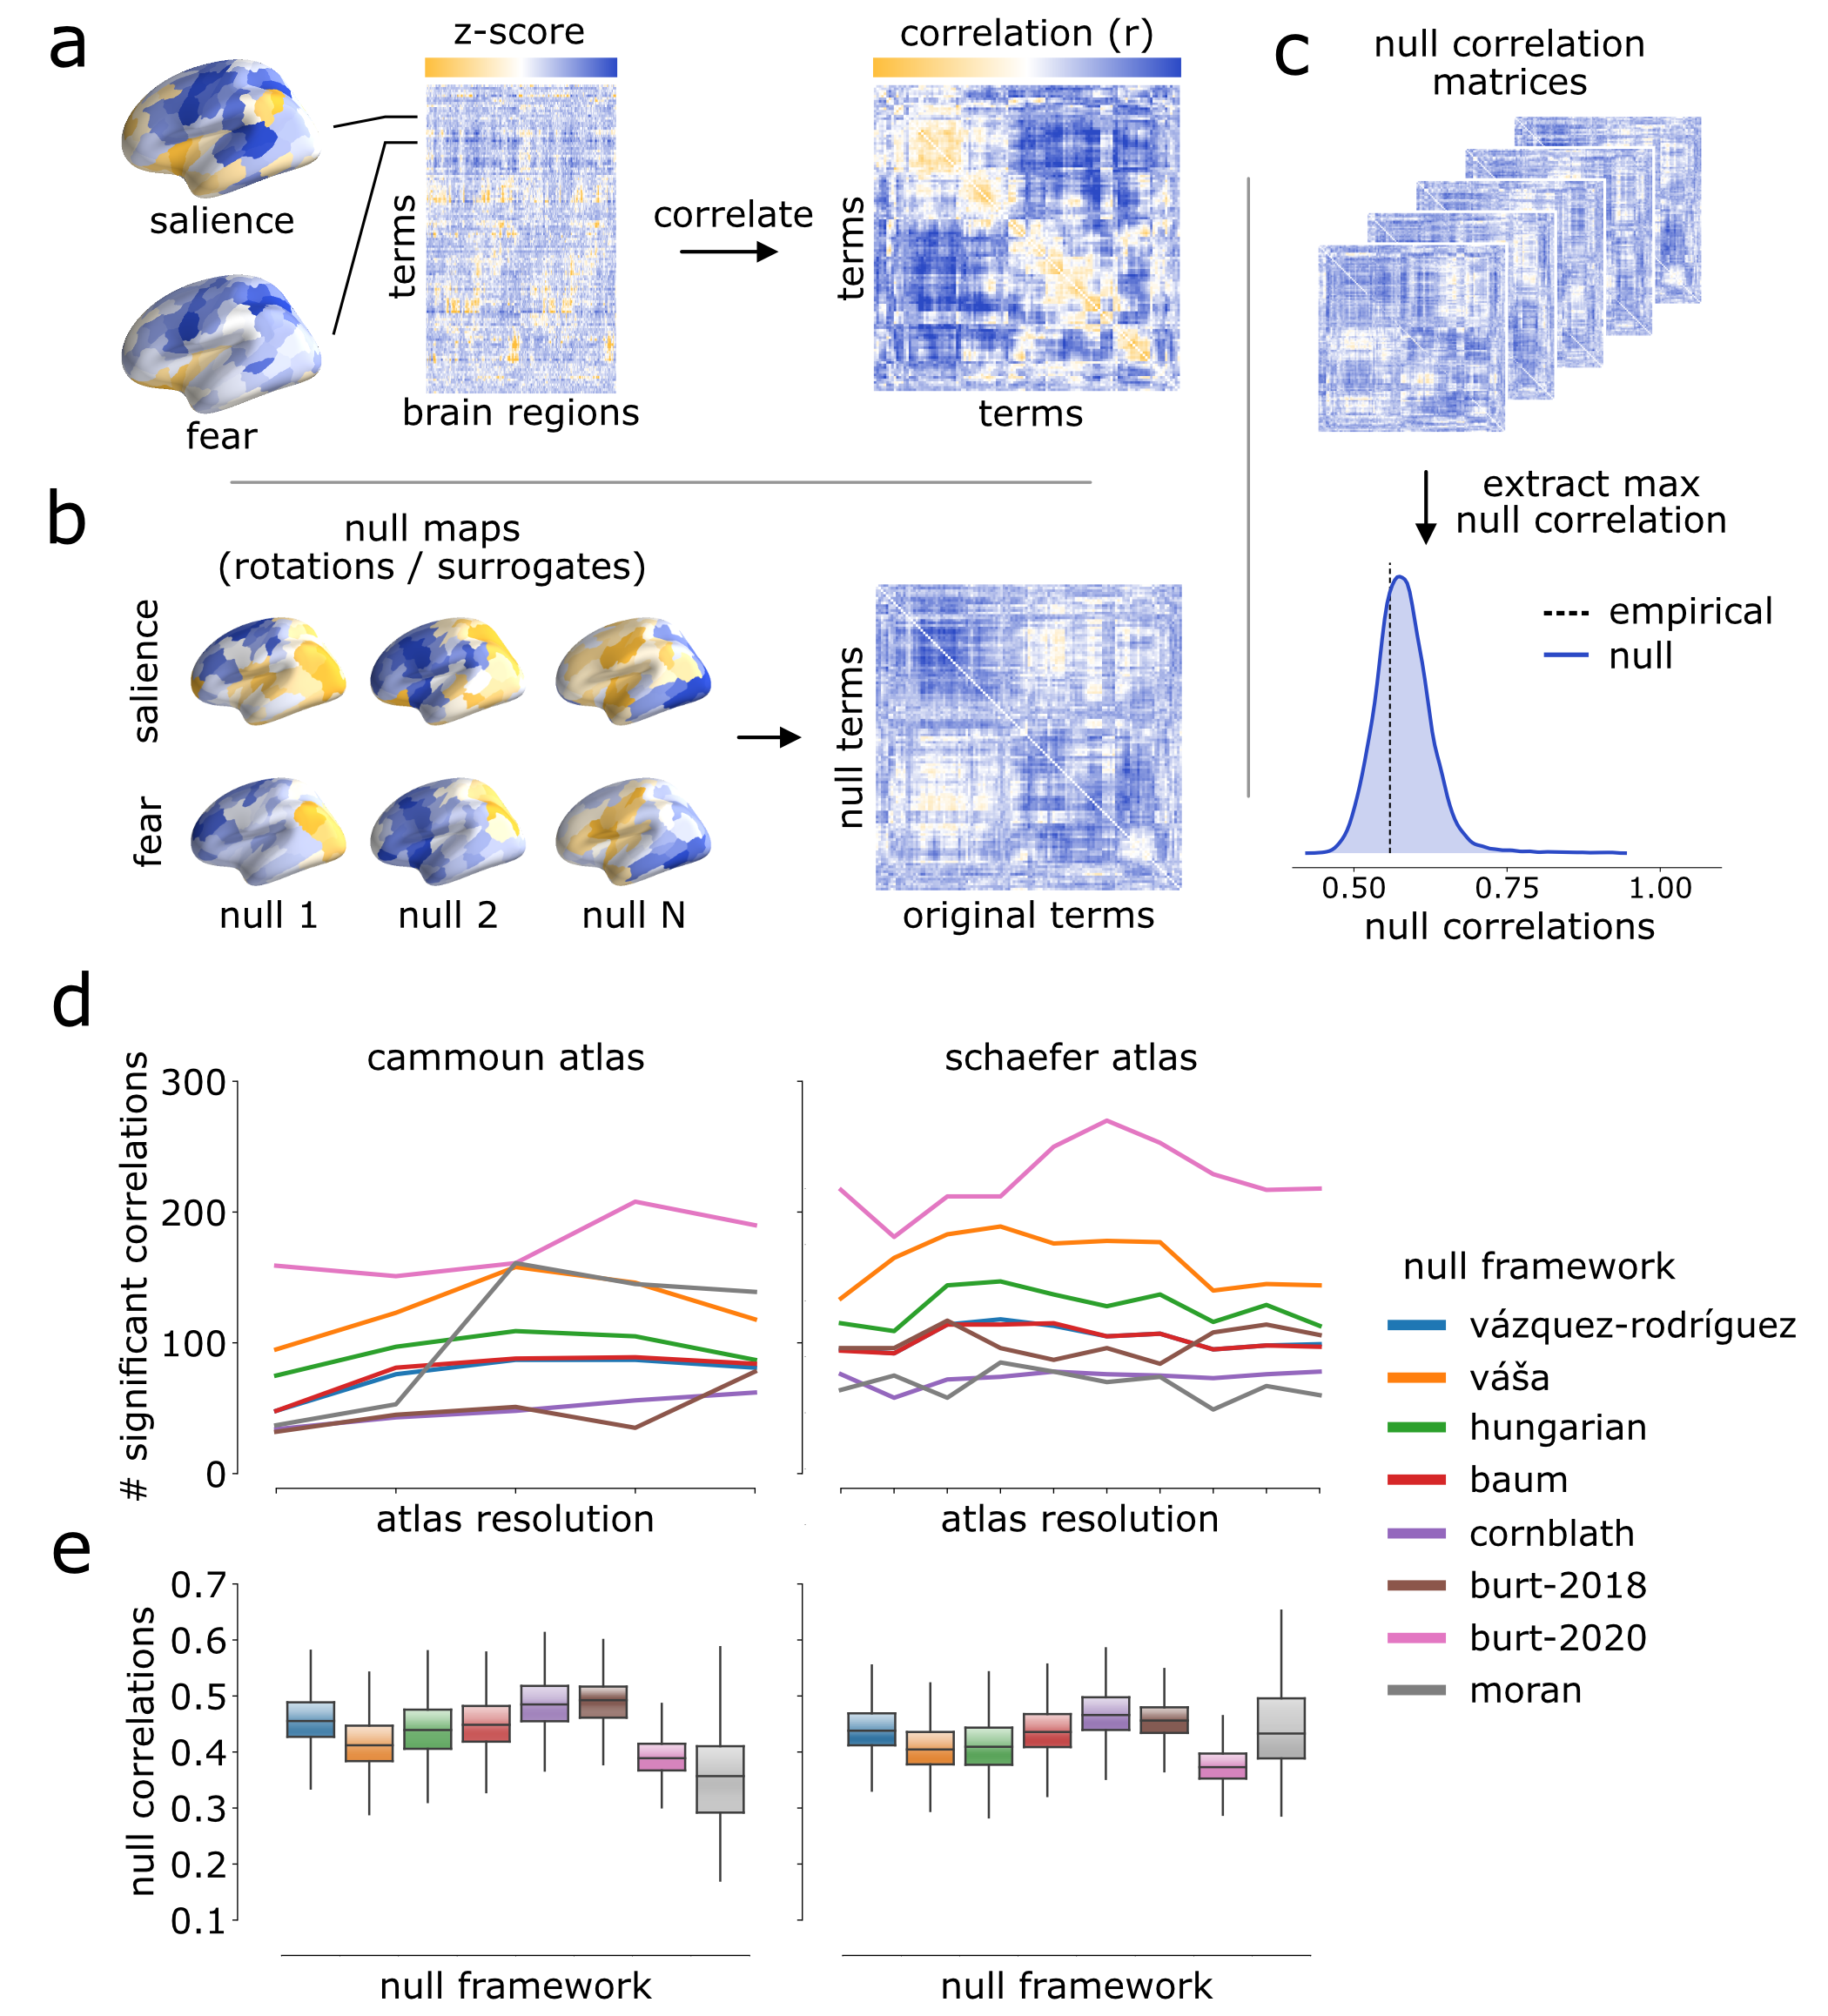
\includegraphics[width=0.95\textwidth]{neurosynth-results.png}}
    \caption{
      \textbf{Testing correspondence between brain maps |}
      (a) ``Association test'' z-score brain maps for 123 terms were downloaded from NeuroSynth.
      The parcellated term maps were correlated across brain regions to generate a term-by-term correlation matrix.
      (b) Each null framework was applied to the original term maps to generate 10,000 null maps per term.
      The original term maps were correlated with each of the null term maps to generate 10,000 null correlation matrices.
      (c) The maximum absolute correlation in each null matrix (excluding the diagonal) was extracted and retained to create a null distribution of correlations.
      This null distribution was used to threshold the original correlation matrix at an alpha of 0.05.
      (d) The number of significant correlations in the thresholded term matrix for each of the null frameworks as a function of atlas and atlas resolution.
      (e) The distributions of null correlations used to threshold the original term correlation matrix.
      Distributions are shown for the highest scale parcellation ($N = 1000$ nodes) of each atlas for all of the null frameworks.
      Refer to Fig.~\ref{supp-figure-naive-nulls}a for spatially-naive nulls and to Table~\ref{supp-table-ns-terms} for a full list of NeuroSynth terms used.
      }
    \label{figure-neurosynth-results}
  \end{center}
\end{figure*}

\subsection*{Null model implementation variability}

While the present report is primarily interested in how the different null models compare to one another, we also wanted to investigate the extent to which methodological choices within each model impact their performance.
That is, most of the null models require researchers to make certain decisions when implementing them in practice.
We investigate two such choices: (1) definition of parcel centroids for the spatial permutation nulls models, and (2) definition of the geodesic distance matrix for parameterized data models.

\subsubsection*{Variability in parcel centroid definition}

We examined the impact of parcel centroid definition on three spatial permutation null models: \textit{V{\'a}zquez-Rodr{\'i}guez}, \textit{V{\'a}{\v{s}}a}, and \textit{Hungarian}.
Parcel centroids were defined using three different techniques operating on the spherical representation of the fsaverage5 surface \citep{fischl1999humanbrainmap}: (1) averaging, (2) surface-projection averaging, and (3) geodesic distance minimization.
In \textit{averaging}, the coordinates for all vertices belonging to a parcel were averaged and used to represent the parcel centroid without further modification \citep{vasa2018cercor}.
Because the vertices are defined on a sphere, these averaged-coordinate centroids will always fall beneath the surface of the cortical mesh.
To resolve this, \textit{surface-projection averaging} performs the same procedure as \textit{averaging} but then selects the coordinates of the closest vertex on the surface of the cortical mesh to represent the parcel centroid \citep{vazquezrodriguez2019pnas}.
An alternative approach, \textit{geodesic distance minimization}, calculates the vertex-by-vertex geodesic distance matrix separately for each parcel.
Each distance matrix is averaged across columns and the coordinates of the vertex with the smallest average is used to represent the parcel centroid.

We generated ten sample reassignments for all nine combinations of parcel centroid definition method and the three aforementioned spatial permutation null models.
The Hamming distance was used to compare the similarity between all generated reassignments \citep{hamming1950distance}.

\subsubsection*{Geodesic distances along the medial wall}

We also investigated the degree to which constraining calculation of surface-based distance matrices to disallow travel along the medial wall impacts the outcomes of parameterized data models.
We generated two distance matrices for each parcellation and resolution, either (1) permitting or (2) disallowing the travelled paths to intersect the medial wall.
Surface distance between vertices was calculated using Dijkstra's algorithm on a graph representing the pial cortical mesh of the fsaverage5 surface \citep{fischl1999humanbrainmap}.
Parcel-to-parcel distance was calculated as the average distance between every surface vertex in two parcels.

We used the generated distance matrices to create 1,000 surrogates for each parameterized data method, yielding 6,000 total surrogates (two distance matrices x three parameterized methods), and assessed the similarity of the resulting surrogates within each method using linear correlations.
As the parameterized data models require an input brain map we used the parcellated T1w/T2w data to generate these surrogates.

\section*{RESULTS}

\begin{figure*}[htp]
  \begin{center}
    \centerline{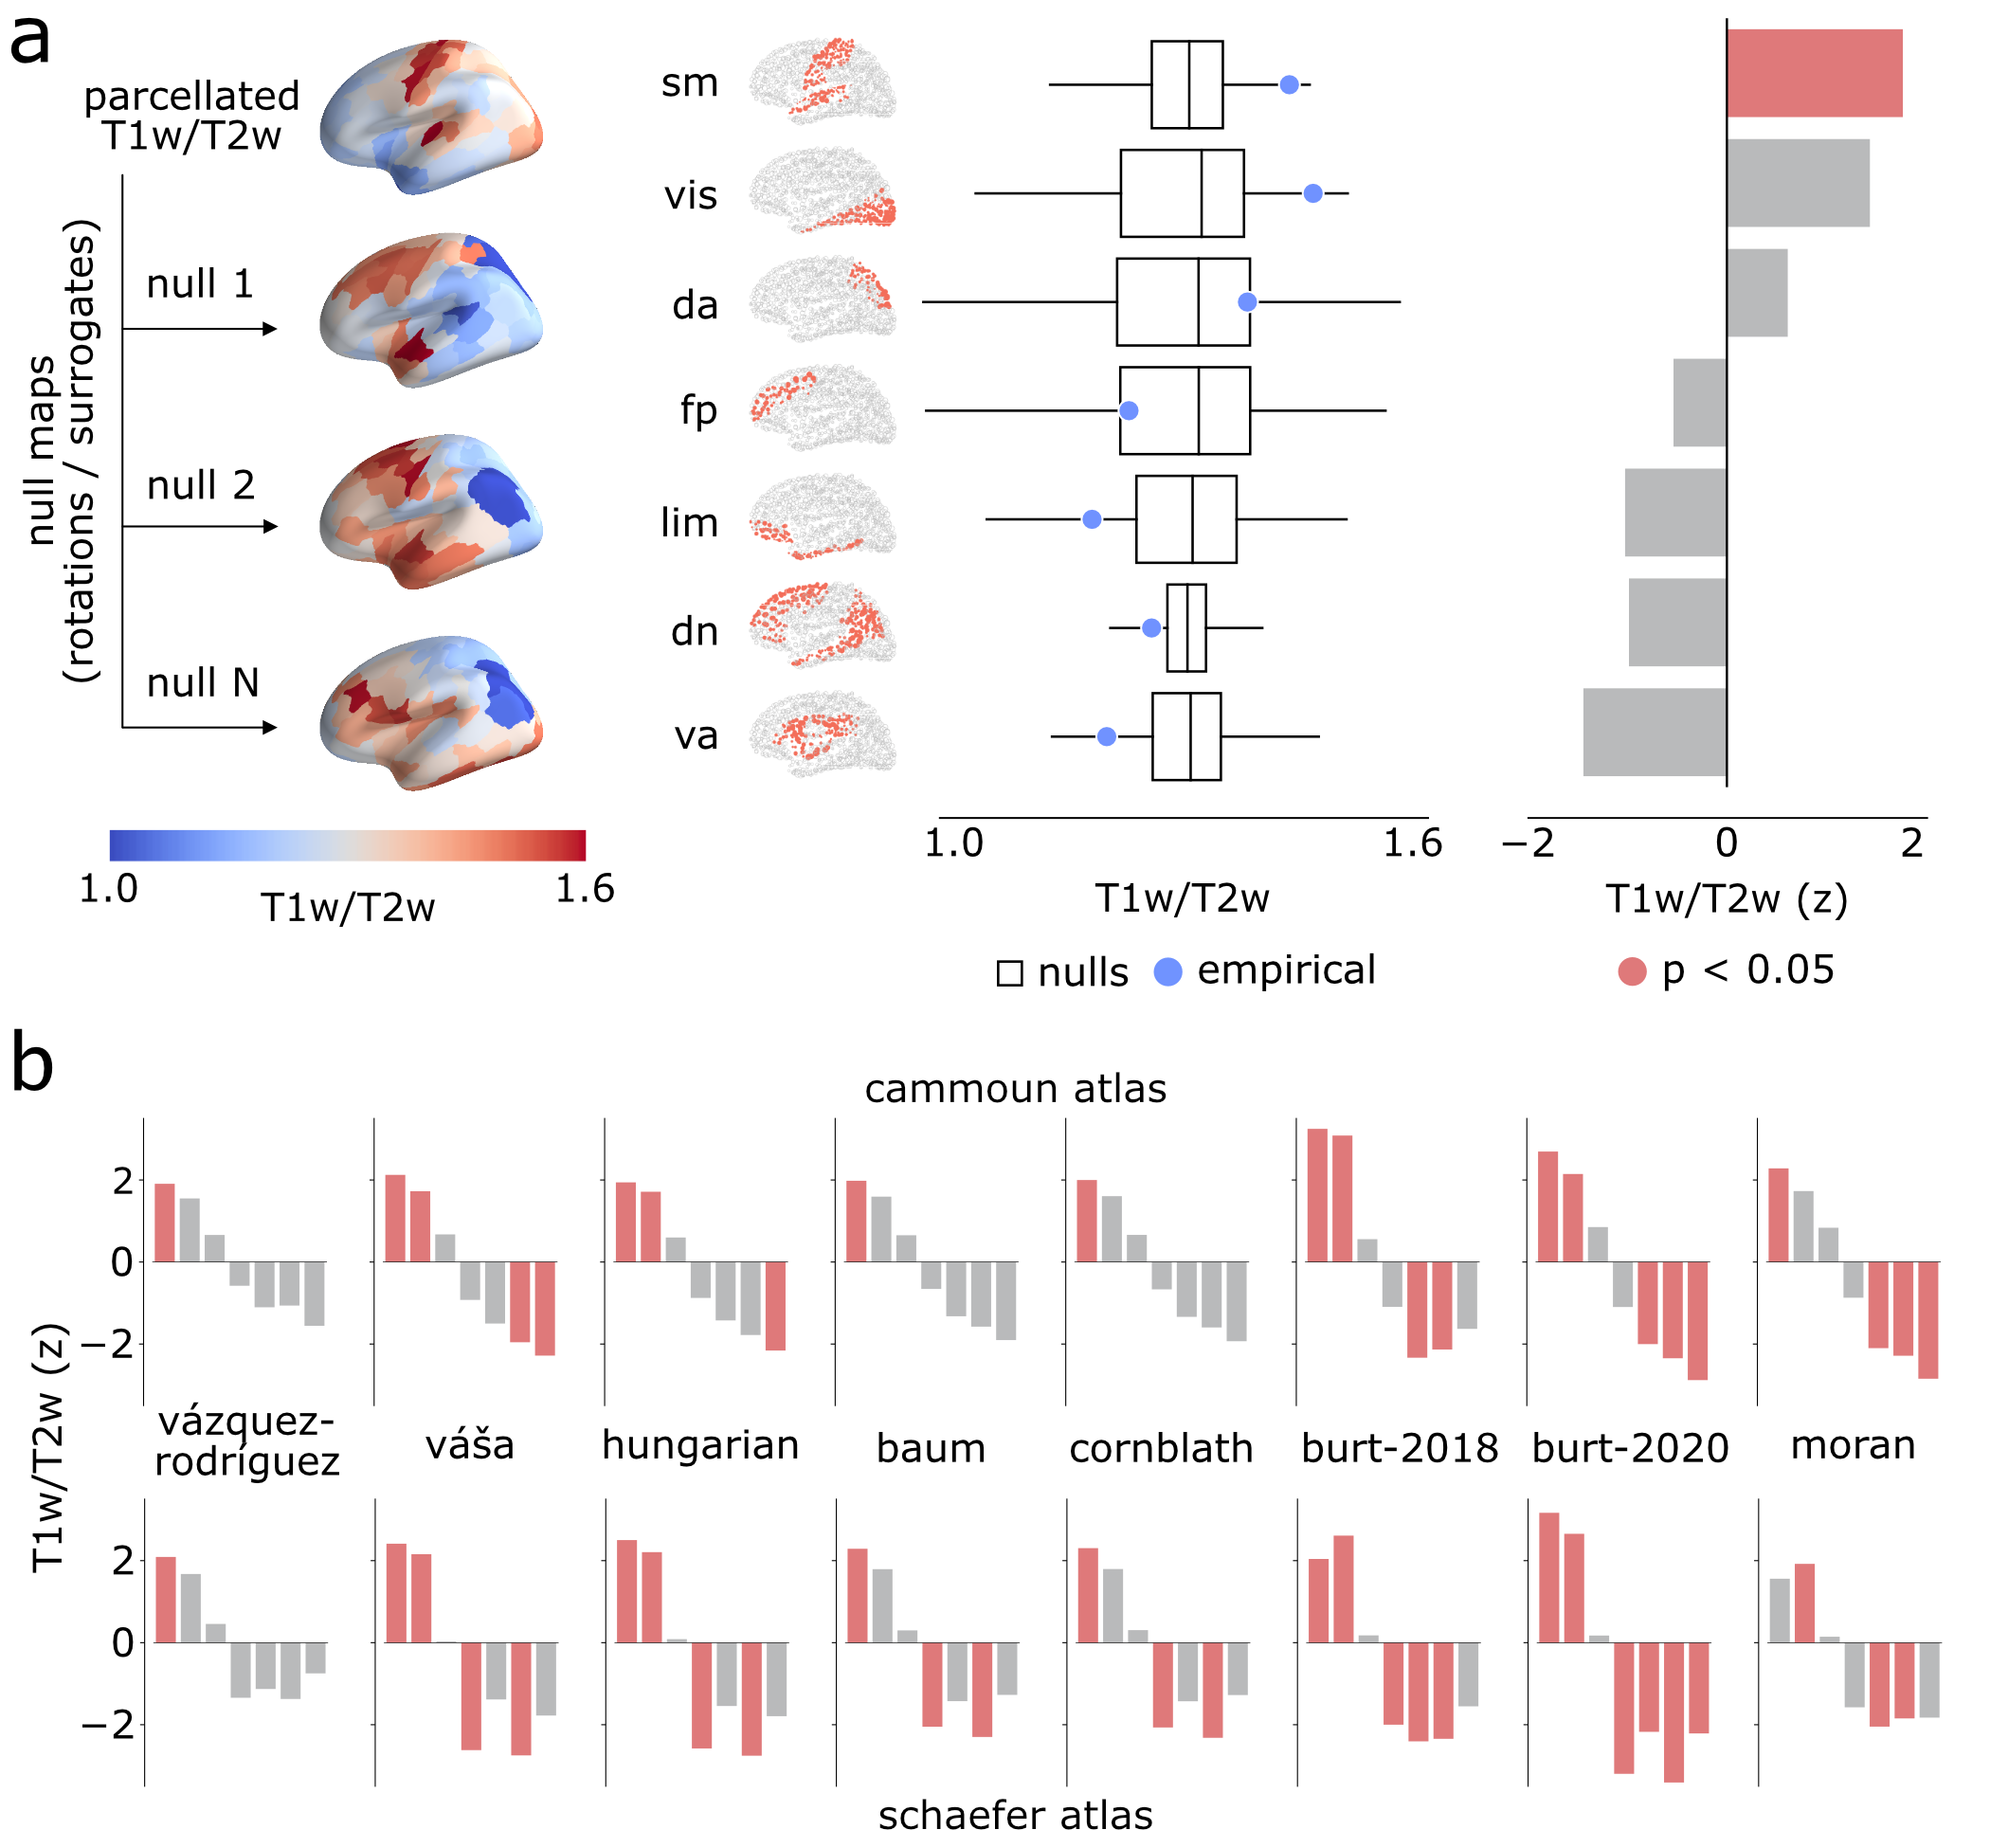
\includegraphics[width=\textwidth]{hcp-results.png}}
    \caption{
      \textbf{Testing partition specificity | }
      (a) Parcellated T1w/T2w data from the Human Connectome Project were subjected to each of the described null frameworks, yielding 10,000 null T1w/T2w brain maps per framework.
      Parcels were averaged within each of the seven Yeo resting state networks \citep{yeo2011organization} for both the empirical (i.e., real) T1w/T2w brain map (blue dot) and the 10,000 null maps for each framework (white boxplot).
      Null distributions were used to normalize the empirical values, yielding a single z-score per network.
      A $p$-value was computed for each network as the proportion of null T1w/T2w network values that exceeded the real T1w/T2w value, divided by the total number of nulls.
      Networks with a $p$-value < 0.05 are shown in red.
      (b) The procedure described in panel (a) was performed for each of the null frameworks for both the Cammoun (top row) and Schaefer (bottom row) atlases.
      Results are shown for the highest scale parcellation ($N = 1000$ nodes) of each atlas.
      Yeo networks are shown from left-to-right in the same top-to-bottom order as in panel (a).
      Network assignments: sm = somatomotor, vis = visual, da = dorsal attention, fp = frontoparietal, lim = limbic, dn = default network, va = ventral attention.
      }
    \label{figure-hcp-results}
  \end{center}
\end{figure*}

We performed two analyses to investigate the impact of ten null models on controlling the FWER in statistical assessments of parcellated brain data.
We briefly describe both analyses below and provide an overview of each of the ten null models in Table~\ref{table-null-models} (refer to \emph{Methods and Materials} for more information; see Fig.~\ref{figure-null-frameworks} for an example null map from each model).

\subsection*{Testing correspondence between brain maps}

We first investigate how each of the ten null models performs in a prototypical correspondence analysis, in which a user assesses the spatial correlation between two brain maps.
As an example, we test correlations between meta-analytic functional activations.
Following \citet{alexanderbloch2018neuroimage}, we parcellated meta-analytic ``association'' maps for 123 cognitive terms derived from NeuroSynth \citep{yarkoni2011natmethods, poldrack2011frontiers}.
We used the term-specific association maps to construct a term $\times$ term linear correlation matrix, indicating the extent to which pairs of terms share a similar spatial pattern (Fig.~\ref{figure-neurosynth-results}a).
We then applied each null model to generate a population of null term $\times$ term correlation matrices (Fig.~\ref{figure-neurosynth-results}b).
Finally, we constructed a null distribution by retaining the maximum absolute correlation coefficient from each of the null term $\times$ term matrices, excluding the diagonal elements (Fig.~\ref{figure-neurosynth-results}c).
This procedure yielded distributions of null correlations for each null model, which were used to threshold the empirical term $\times$ term correlation matrix \citep{alexanderbloch2018neuroimage}.

Figs.~\ref{figure-neurosynth-results}d show the number of statistically significant correlations that remained in the term-by-term matrix after thresholding.
All comparisons were performed at $\alpha=0.05$.
Results are organized according to two commonly-used parcellations of the cerebral cortex grey matter: one anatomical \citep{desikan2006automated, cammoun2012mapping} and one functional \citep{schaefer2018cercor}.
To test the interaction between null model and parcellation resolution, analyses were repeated at multiple resolutions (5 resolutions for the Cammoun Atlas; 10 resolutions for the Schaefer atlas).

Altogether, we find consistent differences between null models (Fig.~\ref{figure-neurosynth-results}d,e and Fig.~\ref{supp-figure-naive-nulls}a).
In particular, some of the methods are more liberal, yielding higher numbers of significant correlations (e.g. \textit{Burt-2020}, \textit{V\'a\v{s}a}), while others are consistently more conservative (\textit{Burt-2018}, \textit{Cornblath}).
Interestingly, these differences across null models do not appear to break down according to null model ``family'', with instances of spatial permutation and parameterized data nulls appearing as both more conservative and more liberal.
Moreover, although there are differences among null models, the relative ordering of the null models is stable across multiple parcellation atlases and resolutions, suggesting that models perform consistently across multiple node definitions.

\subsection*{Testing partition specificity}

We next compare null models on tests of partition specificity, in which a user examines whether a spatial feature (e.g. cortical thickness, intracortical myelin, functional connectivity strength) is significantly more concentrated in a partition of interest (e.g. in a specific intrinsic functional network or cytoarchitectonic class).
Specifically, we tested whether the spatial distribution of the T1w/T2w ratio---thought to reflect intracortical myelin \citep{glasser2011jneuro}---is circumscribed by intrinsic functional \citep{yeo2011organization} or cytoarchitectonic \citep{voneconomo1925cytoarchitecture, scholtens2018neuroimage} network boundaries.

We first calculated the mean T1w/T2w ratio for all constituent parcels in the seven intrinsic networks derived by \citet{yeo2011organization} (Fig.~\ref{figure-hcp-results}a).
We then used each of the null models to generate a distribution of network-specific T1w/T2w means.
Finally, each empirical network mean was expressed as a z-score relative to its respective null distribution.
A network-specific $p$-value was estimated by computing the proportion of absolute-valued null network means that were greater than the absolute-valued empirical network mean (Fig.~\ref{figure-hcp-results}a), quantifying the probability that the T1w/T2w ratio is significantly greater or smaller in a particular network, above and beyond the network's size, symmetry, etc.

Fig.~\ref{figure-hcp-results}b shows network-specific z-scores for T1w/T2w ratios.
Intrinsic networks with statistically significant (two-tailed, $\alpha=0.05$) mean T1w/T2w ratios are shown in red, and non-significant networks are shown in grey.
As described above, we repeated all comparisons for two commonly-used multi-scale parcellations \citep{desikan2006automated, cammoun2012mapping, schaefer2018cercor}.


\begin{figure*}[htp]
  \begin{center}
    \centerline{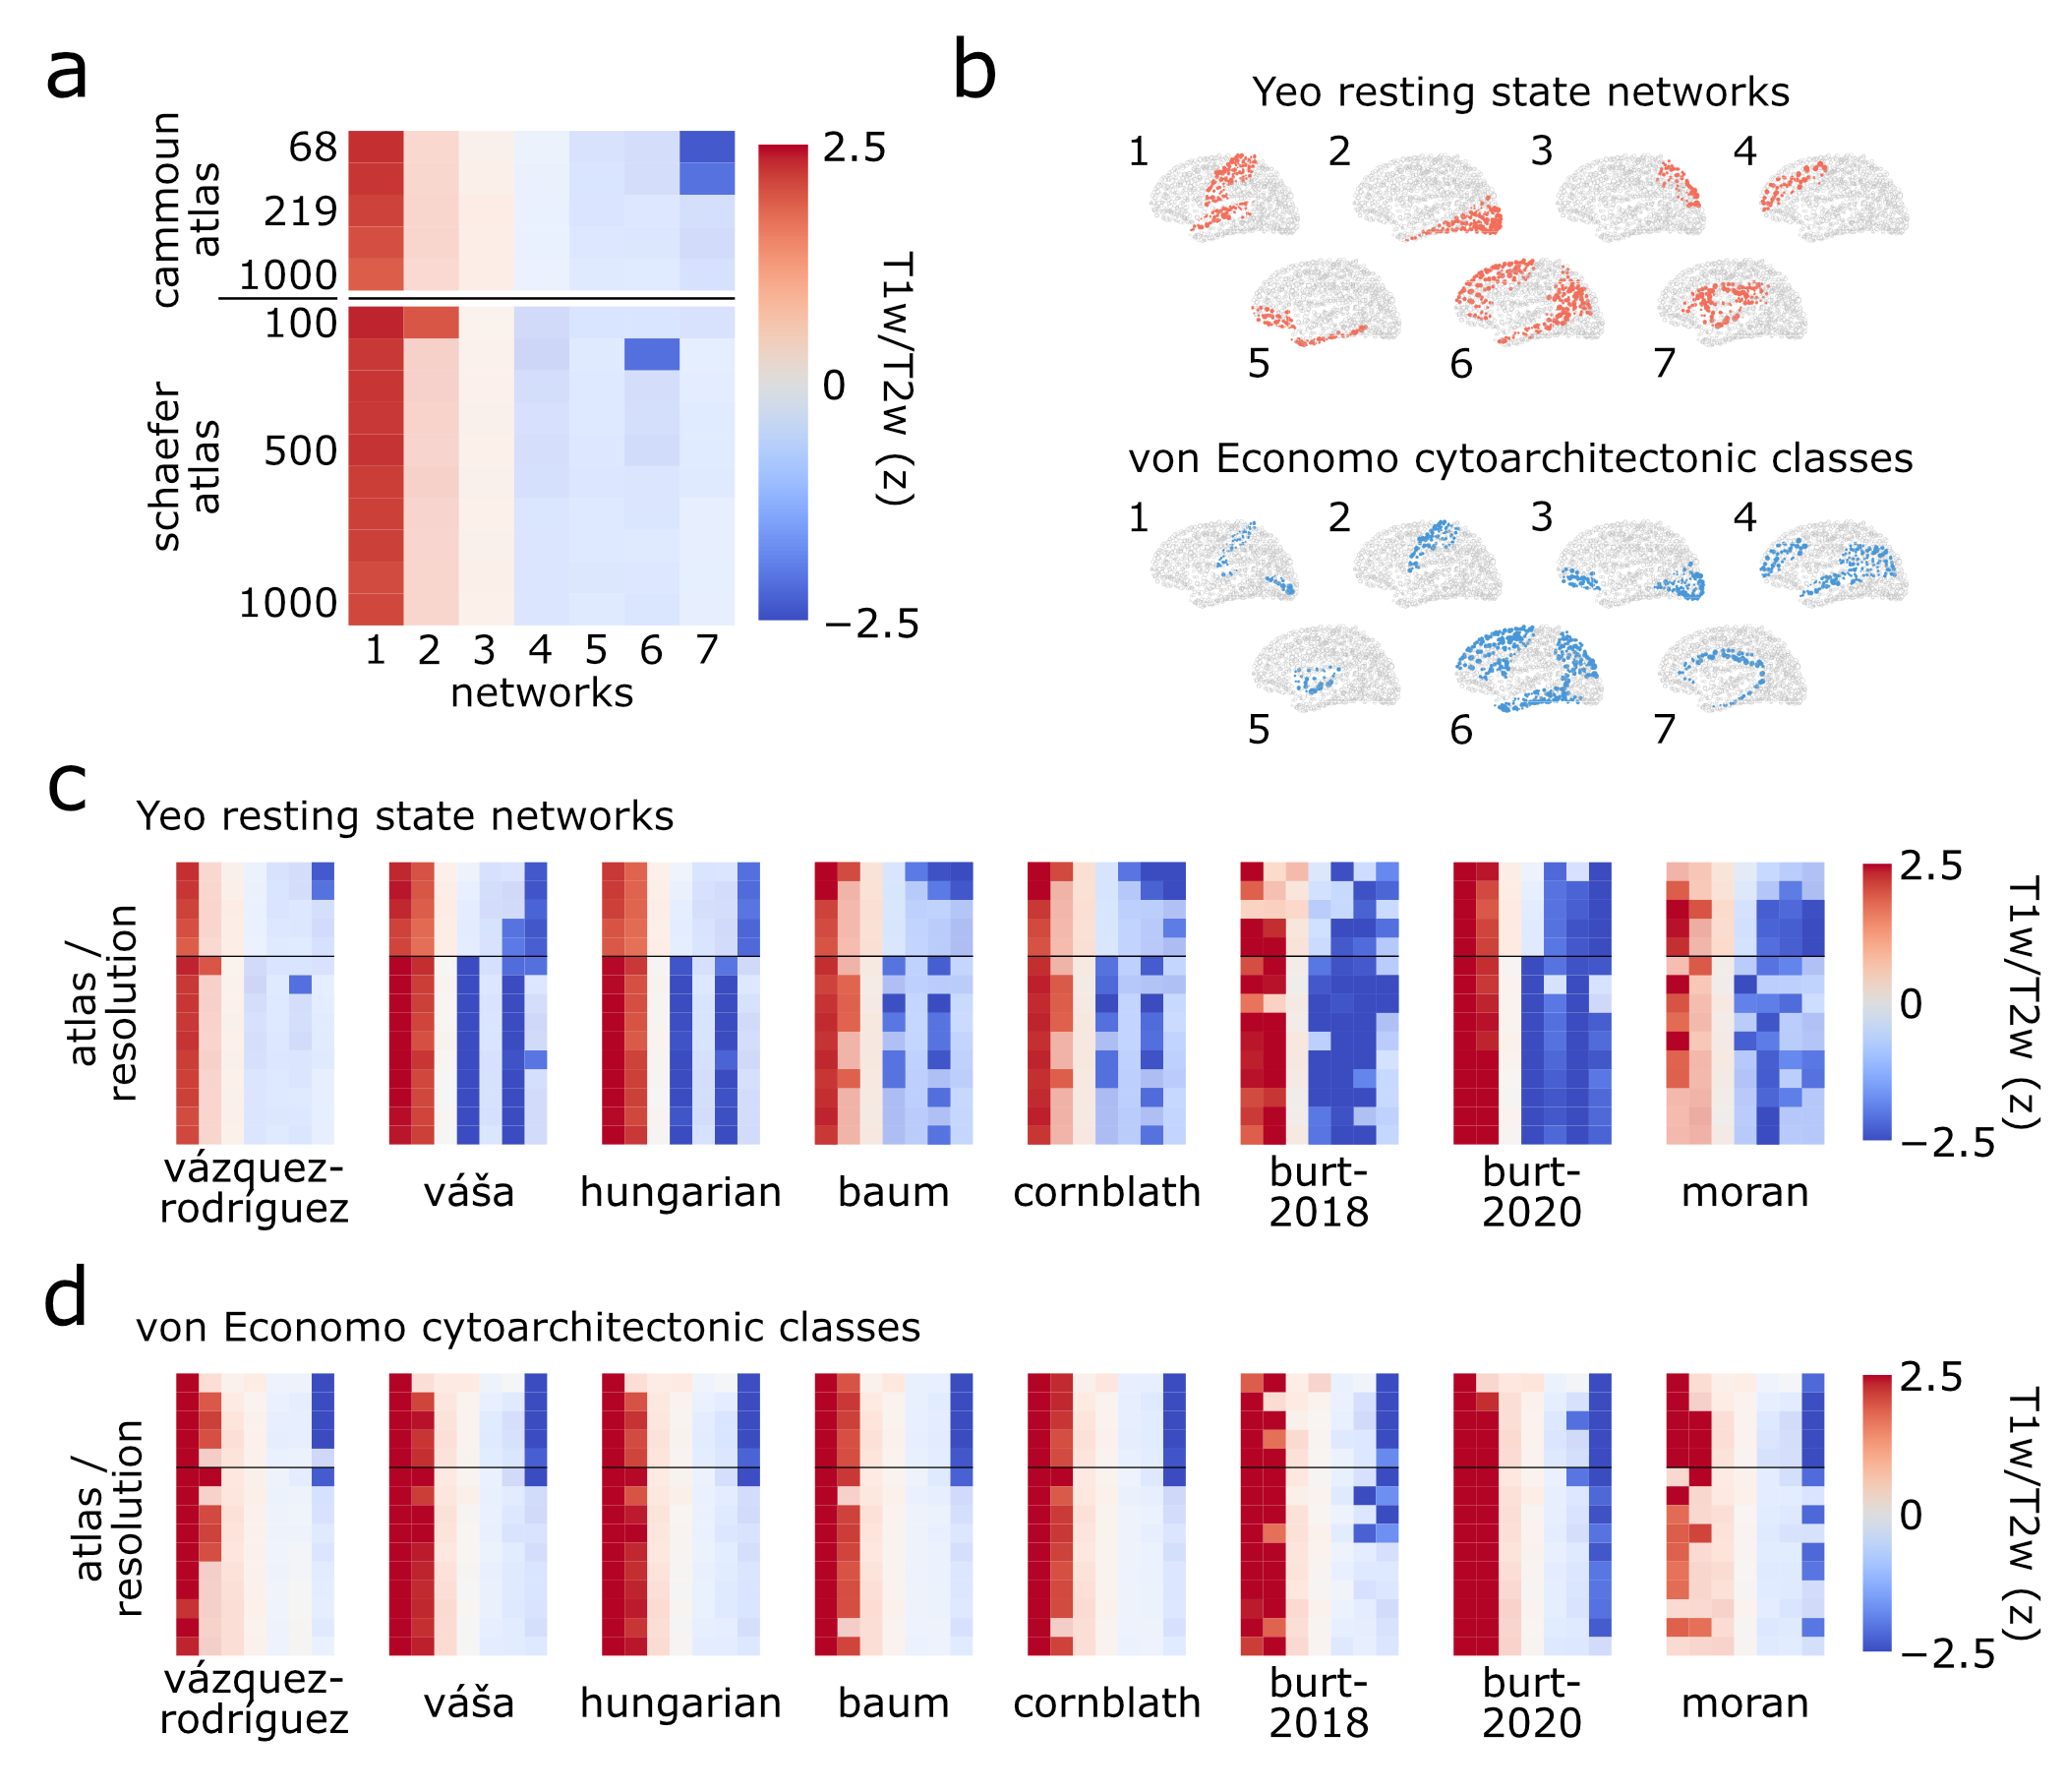
\includegraphics[width=\textwidth]{network-results.png}}
    \caption{
      \textbf{Partition-specific definition of T1w/T2s maps |}
      (a) Overview of the results assessing partition specificity of T1w/T2w measurements.
      Each cell in the heatmap represents the T1w/T2w z-score for a given network (x-axis) and atlas / resolution (y-axis).
      Bold colors represent network z-scores that are significant at the $\alpha = 0.05$ level.
      Note that the fifth and fifteenth row of each heatmap represent the same values shown in Fig.~\ref{figure-hcp-results}b.
      (b) The network labels for both the seven Yeo resting state networks \citep{yeo2011organization} and the seven von Economo-Koskinas cytoarchitectonic classes \citep{voneconomo1925cytoarchitecture, scholtens2018neuroimage}.
      (c, d) The results for all eight spatially-constrained null models for all atlases and resolutions for the (c) Yeo resting state networks and (d) von Economo cytoarchitectonic classes.
      While there is some notable variation amongst atlases and resolutions, primary differences are observable between null frameworks and partitions.
      Refer to Fig.~\ref{supp-figure-naive-nulls}b for spatially-naive nulls.
      Yeo resting state networks: 1 = somatomotor, 2 = visual, 3 = dorsal attention, 4 = frontoparietal, 5 = limbic, 6 = default, 7 = ventral attention.
      von Economo cytoarchitectonic classes: 1 = primary sensory cortex, 2 = primary motor cortex, 3 = primary/secondary sensory cortex, 4 = association cortex, 5 = insular cortex, 6 = association cortex, 7 = limbic regions.
    }
    \label{figure-network-results}
  \end{center}
\end{figure*}

We observe three broad trends.
First, null models are generally consistent in terms of effect direction and relative ordering of network z-scores: most methods identify over-expression of T1w/T2w ratio in the somatomotor and visual networks, and under-expression of T1w/T2w ratios in the ventral attention, default, frontoparietal and limbic networks (Fig.~\ref{figure-hcp-results}b).
Second, despite these similarities, individual null models are inconsistent in the statistical inferences they provide: the number and identity of significant networks varies considerably from model to model.
Third, the models are variable in terms of how conservative they are.
Some models identify only 1/7 significant networks (e.g. \textit{V\'azquez-Rodr\'iguez}), while others identify 6/7 significant networks (e.g. \textit{Burt-2020}, Schaefer atlas).
In contrast to results in the previous section, differences among models appear to break down according to model family, with spatial permutation null models being more conservative (\textit{V\'azquez-Rodr\'iguez}, \textit{Baum}, \textit{Cornblath}) and parameterized nulls more liberal (e.g., \textit{Burt-2018} and \textit{Burt-2020}).

We also investigate differences between parcellation atlas resolutions and network partitions.
Fig.~\ref{figure-network-results}a shows results for a structural and functional atlas (Cammoun and Schaefer) across 5 and 10 resolutions, respectively.
The means are expressed as z-scores relative to a null distribution generated by a given method, and were computed for seven intrinsic functional networks \citep{yeo2011organization}, as well as seven cytoarchitectonic classes \citep{voneconomo1925cytoarchitecture, scholtens2018neuroimage} (Fig.~\ref{figure-network-results}b).
The null model-, atlas-, resolution- and partition-specific z-scores are displayed in Fig.~\ref{figure-network-results}c and d (naive nulls are shown in Fig.~\ref{supp-figure-naive-nulls}b).
Overall, the findings are consistent with the intuitions drawn above.
Namely, we continue to observe consistency across nulls in terms of effect direction and ordering, and inconsistency in the number and identity of significant partitions; however, there is less differentiation between the spatial permutation and parameterized data null models.
Although not specifically related to differences between models, we also note an example of how atlas and partition may potentially interact and lead to different inferences.
Class \#7 of the von Economo partition (limbic regions) is consistently deemed to be significantly under-enriched for T1w/T2w across Cammoun-derived parcellations, while it is generally not statistically significant across Schaefer-derived parcellations (Fig.~\ref{figure-network-results}d).

\begin{figure*}[htp]
  \begin{center}
    \centerline{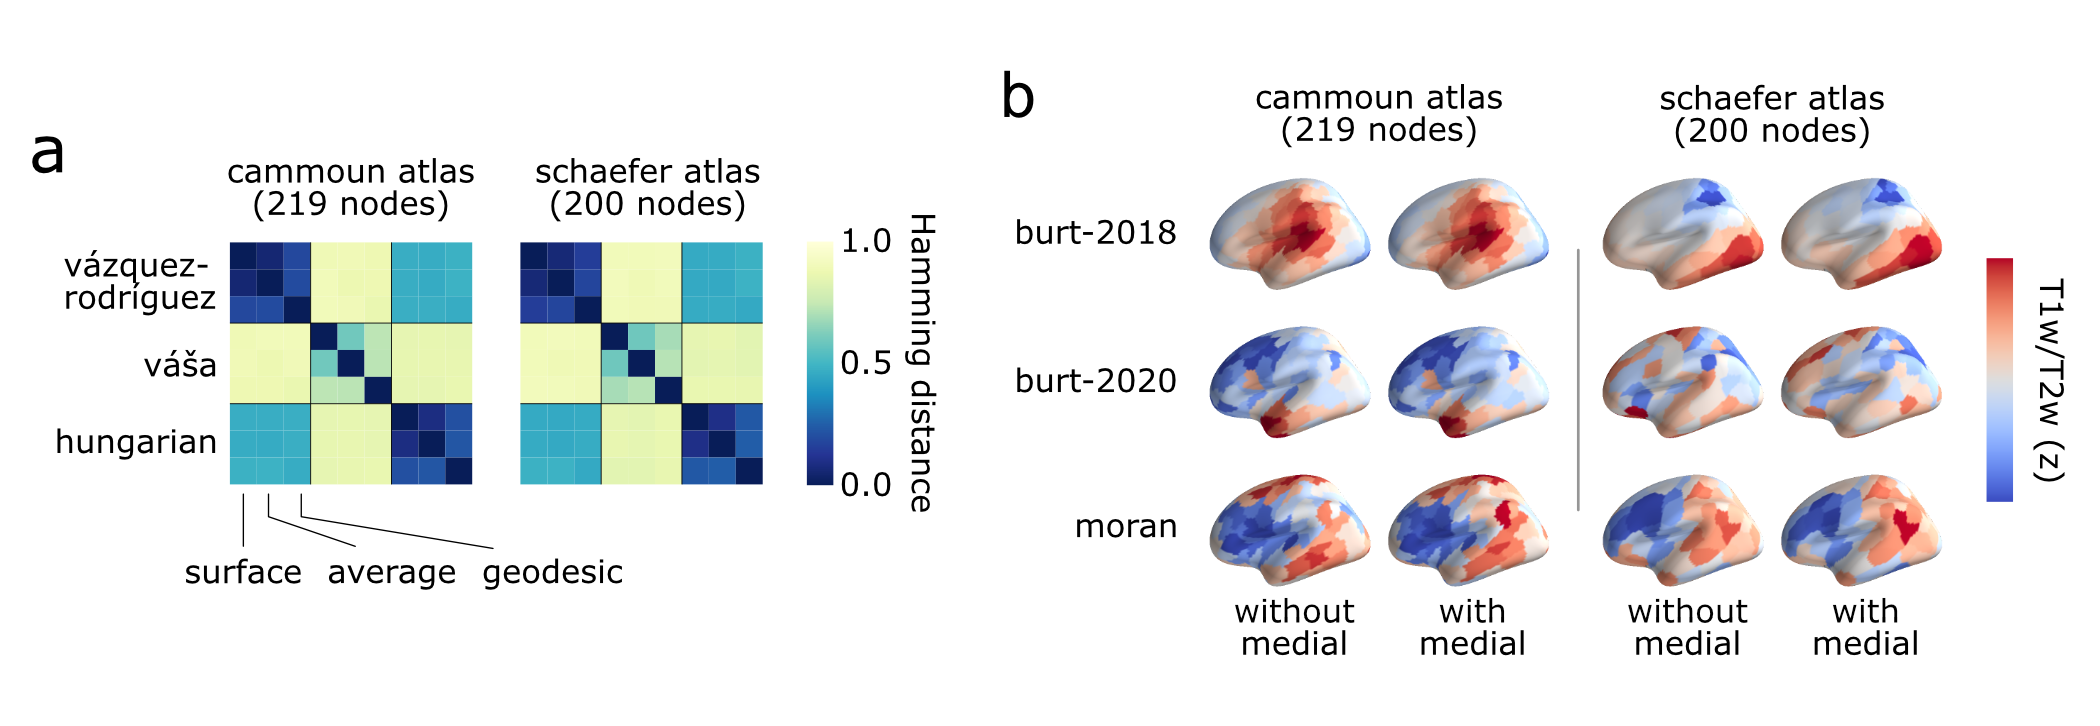
\includegraphics[width=\textwidth]{implementation_differences.png}}
    \caption{
      \textbf{Implementation of null models can impact performance |}
      (a) The impact of parcel centroid definition on three spatial permutation null models.
      Heatmaps show the correspondence (Hamming distance) between null reassignments generated using different null frameworks and parcel centroid methods, where lower values (blue colors) indicate greater correspondence.
      The heatmaps are broken into nine sections (black outlines) which delineate different null frameworks; cells within each section represent the different parcel centroid methods.
      For results from all resolutions of the Cammoun and Schaefer atlases refer to \ref{supp-figure-parcel-centroids}.
      (b) Example surrogates generated from distances matrices allowing (``with medial'') and disallowing (``without medial'') surface distance travel along the medial wall for three parameterized data null models (Burt-2018, Burt-2020, and Moran).
    }
    \label{figure-implementation-differences}
  \end{center}
\end{figure*}

\subsection*{Implementation of null models can impact performance}

While the presented results suggest that, at a broad level, selection of null model framework is an important choice for researchers, it is by no means the only choice that can impact analytical results.
Here, we investigate how different implementations and seemingly minor methodological choices of individual spatial permutation and parameterized data null models can influence statistical outcomes.

\subsubsection*{Variability in parcel centroid definition}

Of the five spatial permutation null models presented in the current report, three require definition of a centroid for each parcel (\textit{V{\'a}zquez-Rodr{\'i}guez}, \textit{V{\'a}{\v{s}}a}, and \textit{Hungarian}).
For the analyses reported, parcel centroids were generated following the procedure used by \citet{vazquezrodriguez2019pnas}, which include: (1) taking the average of the coordinates of all vertices within a given parcel and (2) using the coordinates of the surface vertex closest to this average (where closest is defined as minimizing Euclidean distance).
However, \citet{vasa2018cercor} defined their parcel centroids using only the average of the vertices within each parcel (i.e., not projecting back to a surface vertex).
Notably, both of these procedures fail to take into account oblong or C-shaped parcels for which the center-of-mass may fall outside the boundaries of the parcel.
An alternative approach to account for this possibility is to find the coordinates of the vertex that minimizes the average surface (geodesic) distance to all other vertices within each parcel.

We assessed the extent to which these three different methods of parcel centroid definition impacted the generated rotations for the three relevant null models.
We generated ten rotation matrices and applied them to the coordinates derived from each of these three parcel centroid definition methods, reassigning parcels using the approach from each of the three relevant null frameworks.
We compared the similarity of the reassignments using the Hamming distance (Fig.~\ref{figure-implementation-differences}a; \citealt{hamming1950distance}).
Critically, because the same rotations were applied for every model and method, any observed differences are a result of variation in either the parcel centroid coordinates or models themselves.

Fig.~\ref{figure-implementation-differences}a shows the Hamming distance between reassignments for all combinations of these parcel centroid and null framework methods across the Cammoun and Schaefer atlases (219 and 200 nodes, respectively; refer to \ref{supp-figure-parcel-centroids} for all resolutions).
Predictably, we observe the strongest differences between reassignments generated from the different null methods.
In particular, the \textit{V{\'a}{\v{s}}a} null method seems to markedly differ from the \textit{V{\'a}zquez-Rodr{\'i}guez} and \textit{Hungarian} methods.
In addition, there is also variation between parcel centroid calculation methods; for example, the \textit{V{\'a}{\v{s}}a} method seems to have only moderate correspondence between different parcel centroid definitions.
Altogether, these results highlight important differences not only between spatial permutation null models but within the implementation of each model itself.

\subsubsection*{Geodesic distances along the medial wall}

One notable disadvantage of spatial permutation null models is that the rotations on which they rely will cause the medial wall to be displaced into the cortical sheet (Fig.~\ref{figure-null-frameworks}).
The resulting null distribution will have missing data for this portion of the cortex and discarded data for the cortex rotated into the medial wall, yielding uneven sample sizes between null distributions and potentially biasing results (refer to \citealt{burt2020neuroimage} for an illustration of this concept).

While the family of parameterized data models do not rely on rotations and thus are not subject to this constraint, they do rely on a user-defined weight matrix that provides an estimation of the spatial structure of the related brain maps.
In most cases---as in the current report---this weight matrix takes the form of a geodesic- or surface-based distance matrix calculated from shortest paths taken along the surface mesh projection of a brain.
However, the calculation of these distance matrices often fails to take into account that paths along the brain's medial wall, where the cortical sheet is discontinuous due to underlying white matter and subcortical nuclei, should not be possible.
Failing to account for this discontinuity yields distance matrices that categorically underestimate the actual distance between many brain regions.

We tested the extent to which generating distance matrices (dis-)allowing travel along the medial wall biases the surrogate data maps generated from the three parameterized null models.
Fig.~\ref{figure-implementation-differences}b shows an example surrogate map for these null models for the Cammoun and Schaefer atlases.
Overall, surrogates generated from the different distance matrices show strong similarities.
To examine this in more detail we correlated 1,000 surrogates generated from the two distance matrices for each method, and found relatively moderate to high correspondence: 0.85 $\pm$ 0.27 (\textit{Burt-2018}), 0.85 $\pm$ 0.15 (\textit{Burt-2020}), 0.94 $\pm$ 0.04 (\textit{Moran}) (mean $\pm$ standard deviation across all atlases and resolutions).
Altogether, although parameterized data nulls seem relatively robust to this issue, how to handle the medial wall when constructing the required distance matrices is still an important choice for researchers to make when implementing these models.

\section*{DISCUSSION}

In the present report we systematically assess the effect of ten null frameworks on statistical inference in two prototypical analyses.
Within the spatially-constrained null frameworks we observe limited differences in performance.
Although in some cases there appears to be a primary distinction between the spatial permutation and parameterized families---with the former tending to be more conservative and the latter more liberal---this strongly depends on research context and question.
Encouragingly, we find minimal impact of parcellation and parcel resolution on these null frameworks.
Across all of our analyses, however, we find that spatially-naive nulls models consistently yield both unrealistically liberal statistical estimates and a strong dependence on parcel resolution, confirming previous reports that these methods are unsuitable for most neuroimaging analyses \citep{alexanderbloch2018neuroimage, burt2020neuroimage}.

From the perspective of a researcher, the first choice when applying one of these frameworks is which family to choose from (Tables~\ref{table-null-models} and \ref{supp-table-null-drawbacks} provide summaries of their relative differences and limitations).
On the one hand, the spatial permutation null models are computationally-efficient.
Since they are not conditioned on the data itself---simply the geometry of the cortical surface---the same null can be applied to any dataset defined on the same cortical mesh.
On the other hand, nulls generated by the parameterized models (with the exception of the Moran method), are dependent on the data itself, dramatically increasing the computational cost for multivariate analyses.
However, the benefit of parameterized nulls is that they can be used for all data geometries.
That is, they can be applied to both volumetric and surface data, and the models are consistent regardless of whether the data are defined at the vertex-, voxel-, or parcel-level \citep{burt2020neuroimage}.

Implementation differences within null families entail additional methodological choices that can ultimately lead to variability in statistical inference (Table~\ref{table-null-models}).
Within the spatial permutation nulls, differences are primarily driven by handling of the medial wall (i.e., \textit{V{\'a}zquez-Rodr{\'i}guez}, \textit{V{\'a}{\v{s}}a}, \textit{Hungarian}) and whether to project parcellated data to the vertex-level (i.e., \textit{Baum}, \textit{Cornblath}).
The parameterized nulls mostly vary in how they implement the data-generating process.
More specifically, these frameworks differ in their underlying assumptions of the nature of the spatial autocorrelation itself and how it is estimated in the first place.
Our results clearly show that these implementation differences have an observable effect on generated statistical estimates, but more research is needed to better understand how differences in performance arise from specific methodological choices.

More broadly, we find that null framework performance depends on the research question itself, such that differences between frameworks are more pronounced for some types of analyses than others.
In particular, we see greater variability between nulls when examining partition specificity (Fig.~\ref{figure-hcp-results}) as compared to brain map correspondence (Fig~\ref{figure-neurosynth-results}).
Within partition specificity analyses we observe increased variability between frameworks when comparing intrinsic resting state networks than when examining cytoarchitectonic classes (Fig~\ref{figure-network-results}).
Indeed, the main limitation of the present report is that it is focused on single instances of two prototypical analyses.
That is, we sample only a small space of the application of these null frameworks and do not exhaustively assess their performance in all conceivable research contexts.

Interestingly, we find that parcellation and parcel resolution seem to have minimal effect on null framework performance.
How brain regions are defined and ultimately represented in analyses is becoming an increasingly important choice in neuroimaging \citep{eickhoff2018natrevneuro}.
Recent work has highlighted the role of brain region definition in analyses including test-retest reliability \citep{arslan2018neuroimage}, structure-function coupling \citep{messe2020hbm, vazquezrodriguez2019pnas}, individual fingerprinting \citep{finn2015natneuro}, modelling of brain dynamics \citep{proix2016neuroimage}, and prediction of behavior and disease \citep{kong2019spatial, dadi2020neuroimage}.
Although the choice of parcellation is clearly an important methodological consideration, our results suggest that it does not strongly influence spatially-constrained null models.
This ostensible ``parcellation invariance'' is encouraging, and will hopefully support broader adoption of these models in future studies.

More generally, this investigation builds on increasing efforts in the neuroimaging literature to benchmark the effects of methodological choices.
Recently, the broad impacts of these choices has been demonstrated in structural MRI \citep{bhagwat2020biorxiv, kharabian2020influence}, task fMRI \citep{carp2012plurality, botviniknesser2020nature}, resting state fMRI \citep{parkes2018neuroimage, ciric2017neuroimage}, and diffusion MRI \citep{oldham2020biorxiv, maier2017natcomm, schilling2019neuroimage} research.
Concomitant with an increasing awareness of the importance of these choices is a developing trend to share and analyze ``raw'' or un-thresholded brain maps \citep{gorgolewski2015neurovault, witt2020biorxiv}.
Convergence of these trends has naturally opened new research questions that revolve around comparing such brain maps.
Methods that appropriately consider the inherent spatial structure of the brain are thus going to be critical to ensuring valid inferences can be drawn from these lines of inquiry.
The present study is a first step towards better understanding the variable implementation of these statistical methods and ultimately standardizing or synthesizing their application.

Collectively, the present report comprehensively examines ten recently-developed null models for comparing brain maps.
We find relatively consistent performance among the null models that account for spatial autocorrelation; however, we note some differences between nulls that depend on analytic framework.
Our results highlight the need to closely consider the variability across implementation of these null methods and to more explicitly compare their performance across a wider range of research contexts.

\subsection*{ACKNOWLEDGEMENTS}

We thank Laura Su{\'a}rez, Golia Shafiei, Justine Hansen, Vincent Bazinet, Bertha V{\'a}zquez-Rodr{\'i}guez, and Elizabeth DuPre for their comments and suggestions. This research was undertaken thanks in part to funding from the Canada First Research Excellence Fund, awarded to McGill University for the Healthy Brains for Healthy Lives initiative. RDM acknowledges support from the Fonds du Recherche Qu{\'e}bec - Nature et Technologies. BM acknowledges support from the Natural Sciences and Engineering Research Council of Canada (NSERC Discovery Grant RGPIN \#017-04265) and from the Canada Research Chairs Program.

\bibliography{refs}

\clearpage

\beginsupplement

\begin{table*}[htp]
    \caption{
      \textbf{List of terms used in NeuroSynth analyses | }
      Terms that overlapped between NeuroSynth \citep{yarkoni2011natmethods} and Cognitive Atlas \citep{poldrack2011frontiers} corpuses used in the reported analyses.
      For a machine-readable format please refer to \url{https://github.com/netneurolab/markello_spatialnulls}.
    }
    \label{supp-table-ns-terms}
    \setlength{\tabcolsep}{4.5pt}
    \renewcommand{\arraystretch}{1.1}
    \begin{center}
      \begin{tabular}{l l l l l}
        action                  & eating             & insight                & naming                 & semantic memory        \\
        adaptation              & efficiency         & integration            & navigation             & sentence comprehension \\
        addiction               & effort             & intelligence           & object recognition     & skill                  \\
        anticipation            & emotion            & intention              & pain                   & sleep                  \\
        anxiety                 & emotion regulation & interference           & perception             & social cognition       \\
        arousal                 & empathy            & judgment               & planning               & spatial attention      \\
        association             & encoding           & knowledge              & priming                & speech perception      \\
        attention               & episodic memory    & language               & psychosis              & speech production      \\
        autobiographical memory & expectancy         & language comprehension & reading                & strategy               \\
        balance                 & expertise          & learning               & reasoning              & strength               \\
        belief                  & extinction         & listening              & recall                 & stress                 \\
        categorization          & face recognition   & localization           & recognition            & sustained attention    \\
        cognitive control       & facial expression  & loss                   & rehearsal              & task difficulty        \\
        communication           & familiarity        & maintenance            & reinforcement learning & thought                \\
        competition             & fear               & manipulation           & response inhibition    & uncertainty            \\
        concept                 & fixation           & meaning                & response selection     & updating               \\
        consciousness           & focus              & memory                 & retention              & utility                \\
        consolidation           & gaze               & memory retrieval       & retrieval              & valence                \\
        context                 & goal               & mental imagery         & reward anticipation    & verbal fluency         \\
        coordination            & hyperactivity      & monitoring             & rhythm                 & visual attention       \\
        decision                & imagery            & mood                   & risk                   & visual perception      \\
        decision making         & impulsivity        & morphology             & rule                   & word recognition       \\
        detection               & induction          & motor control          & salience               & working memory         \\
        discrimination          & inference          & movement               & search                 &                        \\
        distraction             & inhibition         & multisensory           & selective attention    &                        \\
      \end{tabular}
    \end{center}
\end{table*}

\begin{table*}[htp]
    \caption{
      \textbf{Null framework limitations | }
      Overview of some of the drawbacks of each of the null frameworks described in the current report.
      Each of the families also suffer from drawbacks impacting all constituent null frameworks (i.e., spatial permutation models can only handle surface data; parameterized models tend to be more computationally complex); refer to \textit{Discussion} for more information.
      \vspace{-0.5\baselineskip}
    }
    \label{supp-table-null-drawbacks}
    \setlength{\tabcolsep}{4.5pt}
    \renewcommand{\arraystretch}{1.25}
    \begin{center}
      \begin{tabular}{p{0.15\linewidth} p{0.78\linewidth}}
                                                                                                                                                                                          \toprule
        \multicolumn{2}{c}{\textbf{Naive models}}                                                                                                                                      \\ \toprule
        \emph{Method}             & \emph{Drawbacks}                                                                                                                                   \\ \midrule
        Parametric                & Assumes errors are \emph{i.i.d.}; does not account for spatial structure                                                                           \\
        Non-parametric            & Does not account for spatial structure                                                                                                             \\ \toprule
        \multicolumn{2}{c}{\textbf{Spatial permutation models}}                                                                                                                        \\ \toprule
        \emph{Method}             & \emph{Drawbacks}                                                                                                                                   \\ \midrule
        V{\'a}zquez-Rodr{\'i}guez & Allows duplicate parcel assignments                                                                                                                \\
        V{\'a}{\v{s}}a            & Generates sub-optimal assignments with respect to global cost                                                                                      \\
        Hungarian                 & Undesirable, high-cost (i.e., distant) assignments can be made to optimize global cost; time consuming for high-resolution atlases                 \\
        Baum                      & Projection to vertices involves upsampling; allows duplicate parcel assignments                                                                    \\
        Cornblath                 & Projection to vertices involves upsampling; null data will not match original due to re-averaging                                                  \\ \toprule
        \multicolumn{2}{c}{\textbf{Parameterized data models}}                                                                                                                         \\ \toprule
        \emph{Method}             & \emph{Drawbacks}                                                                                                                                   \\ \midrule
        Burt-2018                & Assumes exponential distance model provides accurate estimation of $\hat{\rho}$ and $\hat{d_{0}}$ from data                                        \\
        Burt-2020                & Surrogate data can be unbalanced between hemispheres; variogram models may not properly model some spatial distributions                           \\
        Moran                     & Dependent on provided weight matrix, $\mathbf{W}$, which varies based on neighborhood size; tends to yield highly auto-correlated surrogates       \\
      \end{tabular}
    \end{center}
\end{table*}


\begin{figure*}[htp]
  \begin{center}
    \centerline{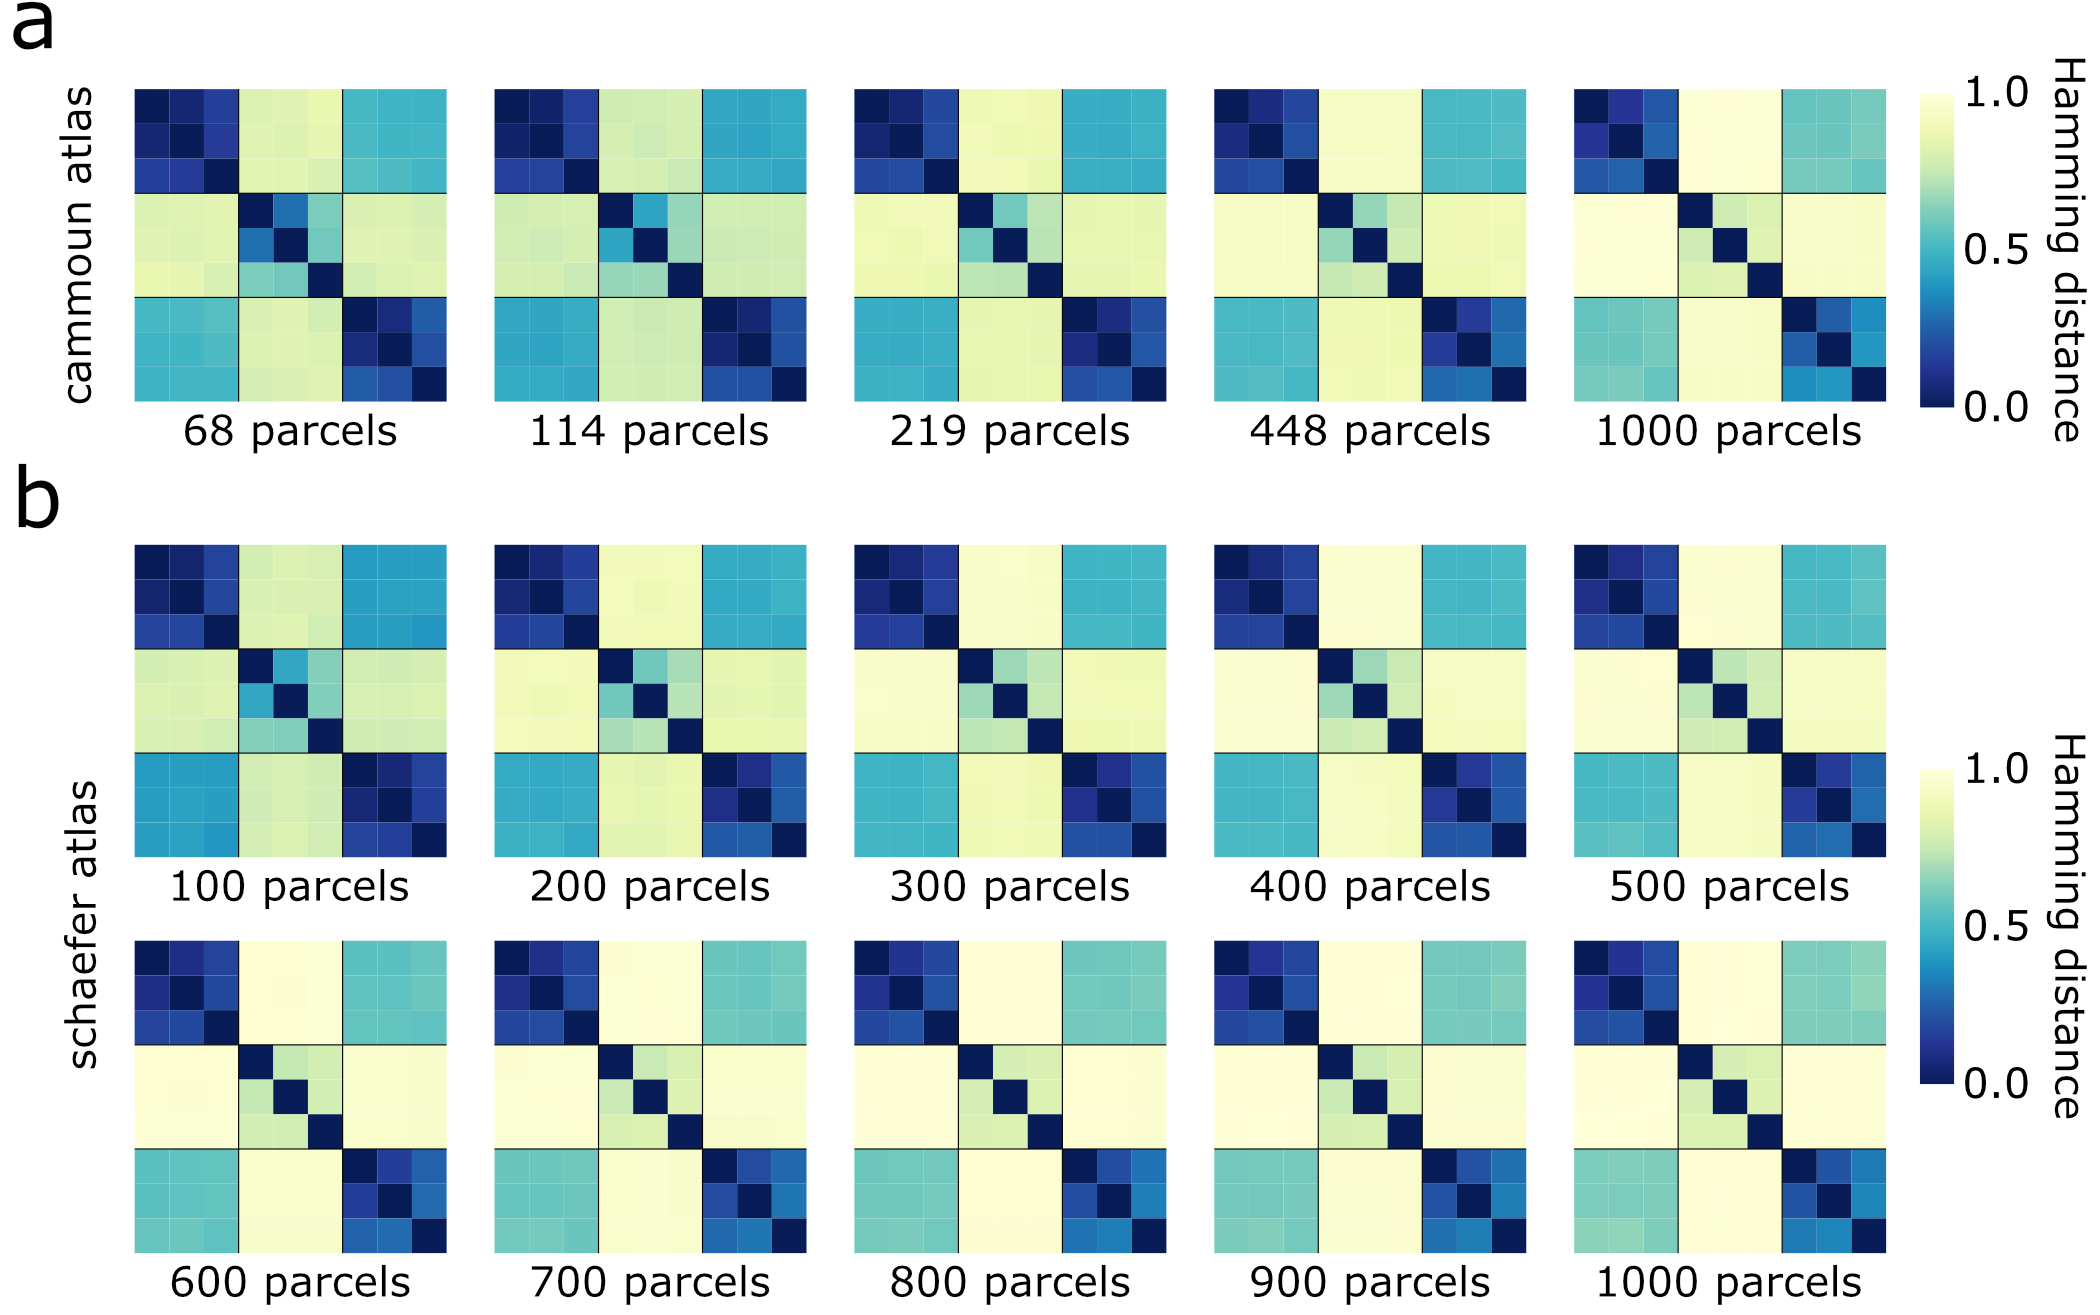
\includegraphics[width=\textwidth]{parcel-centroids.png}}
    \caption{
      \textbf{Variability in parcel centroid definition |}
      Reproduction of results shown in Fig.~\ref{figure-implementation-differences}a for all resolutions of the (a) Cammoun and (b) Schaefer atlases.
      Black lines delineate different null frameworks (\textit{V{\'a}zquez-Rodr{\'i}guez}, \textit{V{\'a}{\v{s}}a}, \textit{Hungarian} from top-to-bottom) and cells within each section of the heatmap represent different parcel centroid definition methods (\textit{surface}, \textit{average}, \textit{geodesic} from top-to-bottom).
      Refer to \textit{Methods and Materials: Null model implementation variability} for more information.
    }
    \label{supp-figure-parcel-centroids}
  \end{center}
\end{figure*}

\begin{figure*}[htp]
  \begin{center}
    \centerline{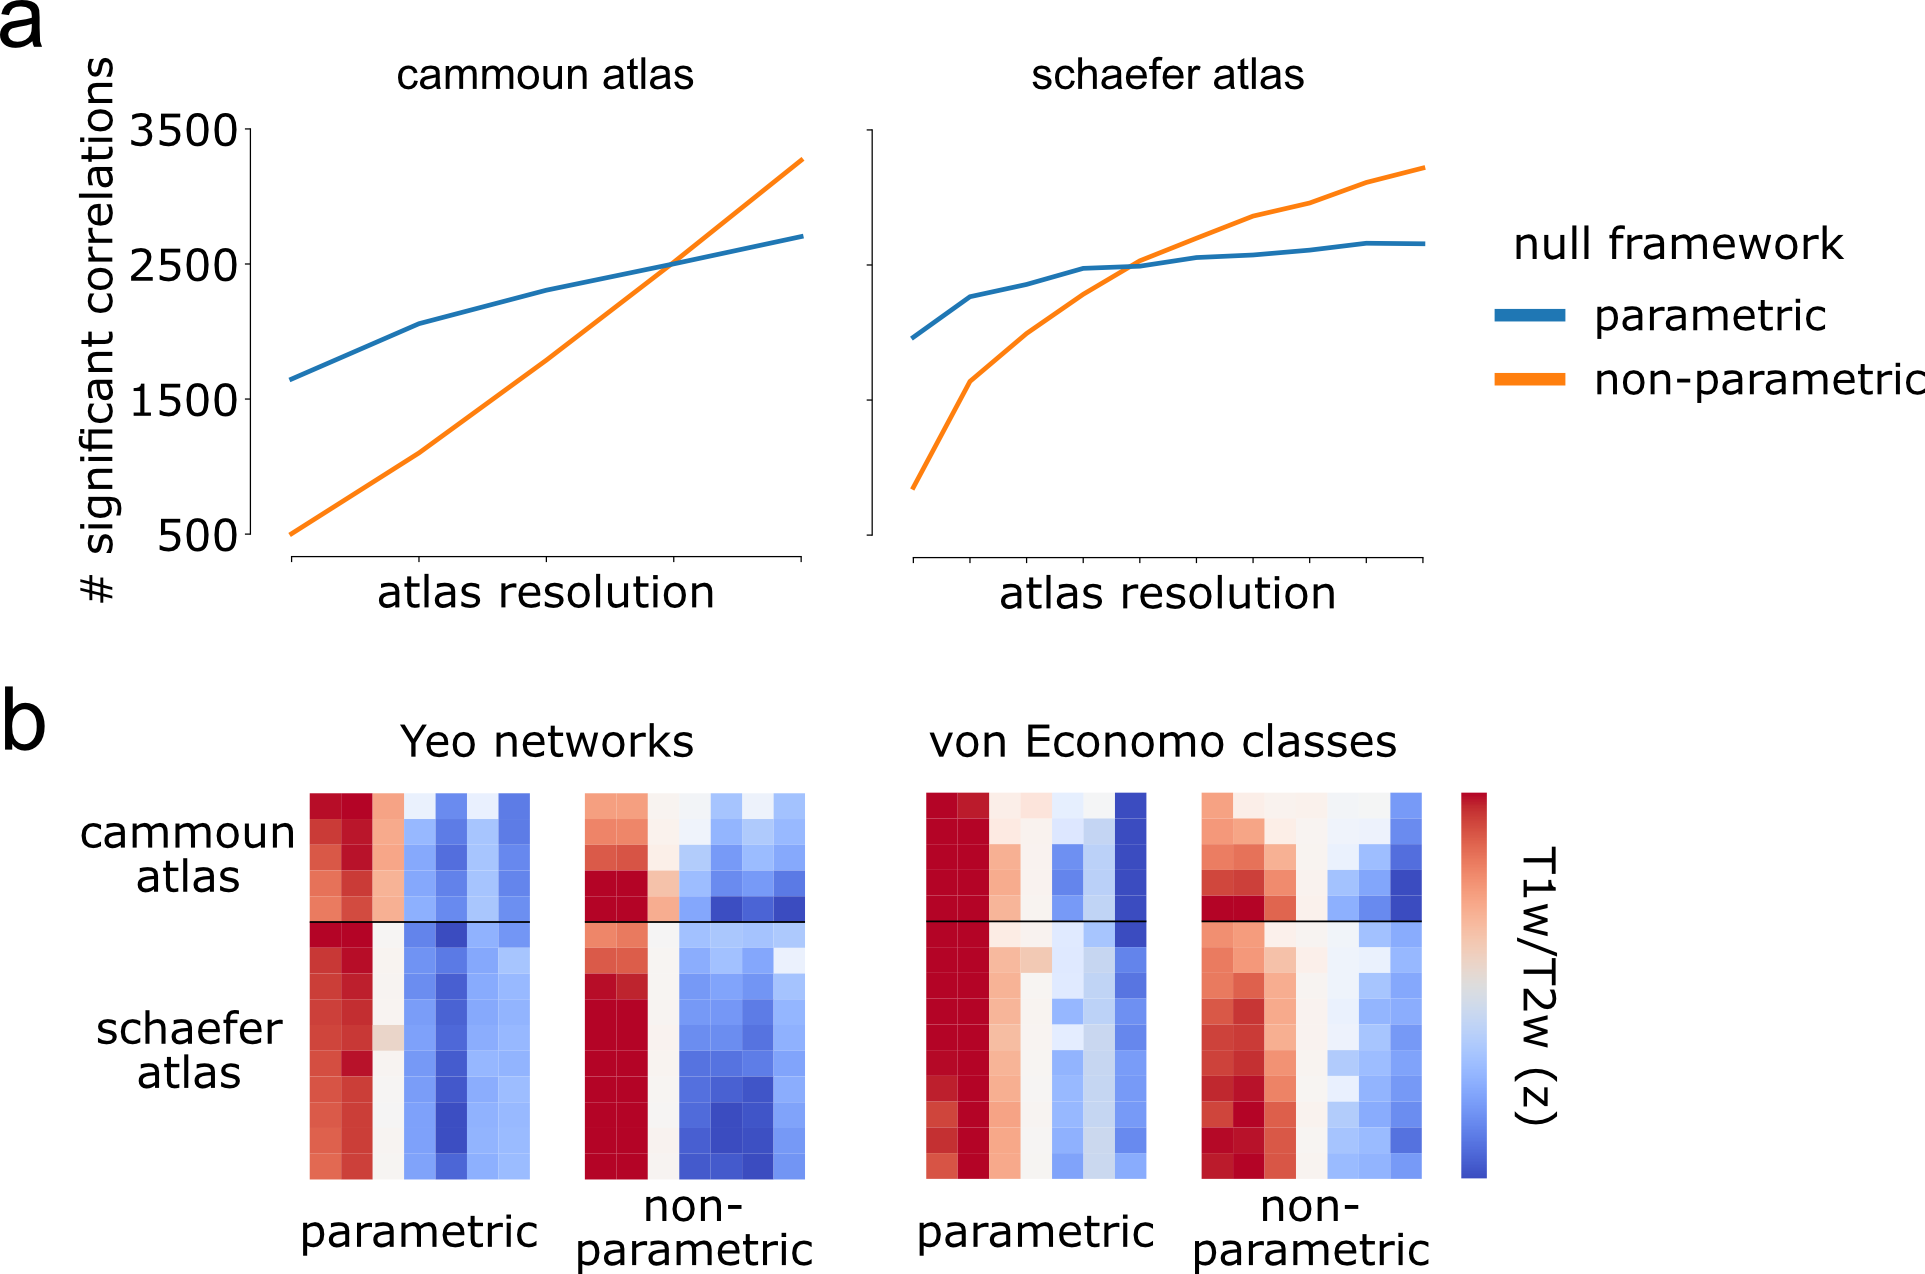
\includegraphics[width=\textwidth]{naive-nulls.png}}
    \caption{
      \textbf{Naive null models |}
      (a) Results of the spatially-naive null models applied to the NeuroSynth analyses described in \textit{Results: Testing correspondence between brain maps}; refer to Fig.~\ref{figure-neurosynth-results} for description of plots.
      Note the different scale of the y-axis as compared to Fig.~\ref{figure-neurosynth-results}d.
      (b) Results of the spatially-naive null models applied to the T1w/T2w analyses described in \textit{Results: Testing partition specificity}; refer to Fig.~\ref{figure-network-results} for description of heatmaps.
      Color scale for \textit{parametric} nulls ranges from -1 to 1 and represents the average T1w/T2w ratio in each network.
      Color scale for \textit{non-parametric} nulls ranges from -7.5 to 7.5 and represents the z-scored T1w/T2w ratio in each network.
    }
    \label{supp-figure-naive-nulls}
  \end{center}
\end{figure*}

\end{document}
